% upon AAS submission
%\documentclass[12pt,twocolumn,tighten,linenumbers]{aastex63}
%\documentclass[12pt,twocolumn,tighten,linenumbers,trackchanges]{aastex63}
% drafting / arxiv
\documentclass[11pt,twocolumn,tighten]{aastex63}
\turnoffedit

\usepackage{apjfonts}
\usepackage{url}
\usepackage{hyperref}
\usepackage{natbib}
\usepackage{amsmath,amstext,amssymb}
\usepackage[caption=false]{subfig} % for subfloat
\usepackage{xcolor, fontawesome}
\usepackage{color}
\usepackage{enumitem}

\newcommand{\red}{\color{red}}

\newcommand{\rprs}{{$R_p/R_{\star}$}}
\newcommand{\vsini}{{$V \sin i$}}
\newcommand{\kms}{{km\,s$^{-1}$}}
\newcommand{\gcc}{{g\,cm$^{-3}$}}
\newcommand{\rstar}{{$R_\star$}}
\newcommand{\rhostar}{{$\rho_\star$}}
\newcommand{\mearth}{{M$_\oplus$}}
\newcommand{\rearth}{{R$_\oplus$}}
\newcommand{\rsun}{{$R_\odot$}}
\newcommand{\msun}{{$M_\odot$}}
\newcommand{\bprp}{G_{\rm BP} - G_{\rm RP}}

\newcommand{\minus}{\scalebox{0.5}[1.0]{$-$}}

\newcommand{\mstype}{letter}

%%%%%%%%%%%%%%%%
% INSTITUTIONS %
%%%%%%%%%%%%%%%%
\newcommand{\caltech}{Department of Astronomy, MC 249-17, California Institute of Technology, Pasadena, CA 91125, USA}
\newcommand{\mitkavli}{MIT Kavli Institute and Department of Physics, 77 Massachusetts Avenue, Cambridge, MA 02139}
\newcommand{\berkeley}{Astronomy Department, University of California, Berkeley, CA 94720, USA}
\newcommand{\princeton}{Department of Astrophysical Sciences, Princeton University, 4 Ivy Lane, Princeton, NJ 08540, USA}
\newcommand{\esa}{European Space Agency (ESA), European Space Research and Technology Centre (ESTEC), Keplerlaan 1, 2201 AZ Noordwijk, Netherlands}
\newcommand{\howard}{Department of Physics and Astronomy, Howard University, Washington DC, 20059}
\newcommand{\goddard}{Center for Research and Exploration in Space Science and Technology, and X-ray Astrophysics Laboratory, NASA/GSFC, Greenbelt, MD 20771, USA}

%
% ms specific numbers
%

%%%%%%%%%
% STARS %
%%%%%%%%%
\newcommand{\nstarssearched}{65760}
\newcommand{\nlcssearched}{180017}


%%%%%%%%
% CRS %
%%%%%%%%

% dip-counting pipeline
\newcommand{\nuniqdipflagged}{{368}} % up-to-date; get_lgb_list_count.py

\newcommand{\ncpvsfound}{70}
\newcommand{\ngoods}{53}
\newcommand{\nmaybes}{17}
\newcommand{\ngoodsfieldbanyan}{three}
\newcommand{\nmaybesfieldbanyan}{0}
\newcommand{\ngoodsnotfieldbanyan}{52}
\newcommand{\nmaybesnotfieldbanyan}{17}
\newcommand{\nnotfieldbanyan}{69}


\begin{document}

%\title{Transient Corotating Clumps Around Adolescent Low-Mass Stars: Four Years of Complex Rotators from TESS}
\title{Transient Corotating Clumps Around Adolescent Low-Mass Stars From Four Years of TESS}


\correspondingauthor{Luke G. Bouma}
\email{luke@astro.caltech.edu}

\received{---}
\revised{---}
\accepted{---}
\shorttitle{Four Years of Complex Rotators} 

\shortauthors{Bouma, Jayaraman, et al.}

%%%%%%%%%%%%%%%%%%%%%%%%%%%%%%%%%%%%%%%%%%
%%%%%%%%%%%%%%%%%%%%%%%%%%%%%%%%%%%%%%%%%%
%%%%%%%%%%%%%%%%%%%%%%%%%%%%%%%%%%%%%%%%%%

% primary authors
\author[0000-0002-0514-5538]{Luke~G.~Bouma}
\altaffiliation{51 Pegasi b Fellow}
\affiliation{\caltech}

\author[0000-0002-7778-3117]{Rahul~Jayaraman}
\affiliation{\mitkavli}

\author{Saul~Rappaport}
\affiliation{\mitkavli}

\author[0000-0001-6381-515X]{Luisa M. Rebull}
\affiliation{\caltech}

\author[0000-0003-4062-0776]{Alexandre David-Uraz}
\affiliation{\howard}
\affiliation{\goddard}

\author{Lynne~A.~Hillenbrand}
\affiliation{\caltech}

\author[0000-0002-4265-047X]{Joshua N. Winn}
\affiliation{\princeton}

\author[0000-0001-7204-6727]{G\'asp\'ar \'A. Bakos}
\affiliation{\princeton}
%
%\author{-----SUGGESTED CONTRIBUTORS, PENDING DISCUSSION, COMMENTS, ANALYSES, ETC-----}
%%
%
%\author[0000-0002-3164-9086]{Maximilian N. G\"unther}
%\affiliation{\esa}
%
%\author[0000-0003-2058-6662]{George~R.~Ricker}
%\affiliation{\mitkavli}



% PENDING DISCUSSION!
%\author[0000-0002-0531-1073]{H. Isaacson}
%\affiliation{\berkeley}
%
%\author[0000-0001-8638-0320]{A. W. Howard}
%\affiliation{\caltech}



%%%%%%%%%%%%%%%%%%%%%%%%%%%%%%%%%%%%%%%%%%
%%%%%%%%%%%%%%%%%%%%%%%%%%%%%%%%%%%%%%%%%%
%%%%%%%%%%%%%%%%%%%%%%%%%%%%%%%%%%%%%%%%%%

% 250 word max!
\begin{abstract}
  We study a set of pre-main-sequence stars
  with sub-solar masses, rotation periods of 0.2--2 days, optical variability amplitudes
  of a few percent, and sharp recurring light curve features that last for
  hundreds of cycles.  The sharp features are probably caused by
  eclipsing clumps of dust or gas orbiting at the corotation radius.
  We refer to this class of variable star as ``complex rotators'' (CRs).
  To improve our understanding of these
  enigmatic objects, we conducted a survey for CRs using TESS
  short-cadence data collected between 2018~July and 2022~September.
  Our search of \nstarssearched\ K and M dwarfs with $T$$<$16 and
  $d$$<$150\,pc yielded \ngoods\ high-quality CRs, most of which are
  new discoveries.  Our sample includes the brightest
  ($T$$\approx$9.5), closest ($d$$\approx$20\,pc), and oldest
  ($\approx$200\,Myr) known CRs.  One of the new discoveries, LP
  12-502, stands out for the complexity of its light curve --- with as
  many as eight flux dips per cycle --- and the detail with which the
  evolution in each dip's amplitude and phase can be tracked over
  1{,}500 cycles.  We argue that corotating gas or dust remains the
  most viable explanation for CRs. The gas or dust is probably
  entrained by the star's magnetic field, and the sharp features may
  result from a multipolar field topology, a hypothesis supported by
  correspondences between the light curves of CRs and of B stars
  known to have strong multipolar magnetic fields.
\end{abstract}


\keywords{Weak-line T Tauri stars (1795),
Periodic variable stars (1213),
Circumstellar matter (241),
Star clusters (1567),
Stellar magnetic fields (1610),
Stellar rotation (1629)}


\section{Introduction}
\label{sec:intro}

\begin{figure*}[!t]
	\begin{center}
		\subfloat{
			\includegraphics[width=0.8\textwidth]{f1a.pdf}
		}
		
		\vspace{-0.65cm}
		\subfloat{
			\includegraphics[width=0.66\textwidth]{f1b.pdf}
		}
	\end{center}
	\vspace{-0.5cm}
	\caption{
		{\bf Complex rotators (CRs)}:
		{\it Top:} Phase-folded TESS light curves for three CRs.  Each
		panel shows the average of the data accumulated over one month,
		relative to the mean stellar brightness.
		Gray circles are raw 2-minute data; black circles are binned to
		300 points per cycle.  The period in hours is printed in the
		bottom right corner.  Left-to-right, the objects are LP 12-502
		(TIC 402980664; Sector~19), TIC 94088626 (Sector 10), and TIC
		425933644 (Sector~28).
		{\it Bottom:} Cartoon explanations for the phenomenon.  The dust
		clump scenario (left) and gas prominence scenario (right) both invoke
		magnetically-entrained corotating material.
	}
	\label{fig:f1}
\end{figure*}

All young stars vary in optical brightness, and the origin of such
variability is, in most cases, understood.  Well-explored sources of
optical variability include inhomogeneities on stellar surfaces such
as starspots and faculae \citep[e.g.][]{2021isma.book.....B},
occultations by circumstellar disks
\citep[e.g.][]{2017MNRAS.470..202B}, and, in geometrically favorable
circumstances, eclipses by stars and planets
\citep[e.g.][]{2020AJ....160...33R}.  More exotic sources of optical
variability that are potentially relevant to this work include
transiting exocomets (e.g.~$\beta$~Pic;
\citealt{2019A&A...625L..13Z}), disintegrating rocky bodies (e.g.
KOI-2700; \citealt{2014ApJ...784...40R}), and occultations by
circumstellar plasma clumps (e.g.~$\sigma$~Ori~E;
\citealt{2005ApJ...630L..81T,2005MNRAS.357..251T}).

Data from K2 \citep{2014PASP..126..398H} and TESS
\citep{2015JATIS...1a4003R} have revealed a new class of variable star
for which the root cause of variability is only beginning to become
clear: complex rotators (CRs).  These objects are identified from
their optical light curves, which show nearly periodic troughs that
are either sharp or broad; these troughs are often superposed on
quasi-sinusoidal spot-like modulation
\citep{2017AJ....153..152S,2018AJ....155...63S,2019ApJ...876..127Z}.
Some CRs show up to eight dips per cycle.  Most CRs are
pre-main-sequence M dwarfs with ages of $\approx$5-150 million years
(Myr), and rotation periods of 0.2--2 days.  They are observed to
comprise $\approx$1-3\% of M dwarfs younger than 100 Myr
\citep{2016AJ....152..114R,2022AJ....163..144G}.  They generally do
not show near-infrared excesses indicative of dusty disks, but the
wavelength-dependent dip amplitudes of some CRs is consistent with
reddening by dust
\citep{2017PASJ...69L...2O,2020AJ....160...86B,2022AJ....163..144G,2023MNRAS.518.2921K}.
The dip amplitudes and phases usually evolve gradually over tens to
hundreds of cycles, although they have occasionally been observed to
change abruptly within one cycle
\citep[e.g.][]{2017AJ....153..152S,2022ApJ...925...75P,2023ApJ...945..114P}.

The sharp features of CR light curves can have durations as short as
5\% of the rotation period ($P_{\rm rot}$), which is too short to be
caused by starspots rotating into and out of view.  Starspots produce
flux variations with characteristic timescales of $P_{\rm rot}$ and
$0.5\,P_{\rm rot}$.  With finely-tuned viewing geometries, starspots
can produce dip durations as short as $\approx$$0.2\,P_{\rm rot}$, but
in such cases, limb darkening causes the dip amplitudes to be smaller
than the observed amplitudes of $\sim$1\% (see
\citealt{2017AJ....153..152S}, Figures 37-41).  Thus, a
``starspot-only'' scenario can be ruled out for many CRs
\citep{2017AJ....153..152S,2019ApJ...876..127Z,2021MNRAS.500.1366K}.
Given that many CRs cannot be explained by starspots alone, and
working under the assumption that all CRs share the same basic
physical scenario, we discard the ``starspot-only'' scenario.
Instead, the correct explanation probably involves material above the
stellar surface that is spatially confined with sharp boundaries
\citep[e.g.][]{2017AJ....153..152S,2022AJ....163..144G}.

Figure~\ref{fig:f1} illustrates two proposed models for the extrinsic
material.  The first scenario invokes opaque dust ``clumps'' that
orbit near the Keplerian corotation radius [$R_{\rm c} =
(GM/\Omega^2)^{1/3}$, where $\Omega = 2\pi/P_{\rm rot}$] and
periodically transit the star
\citep{2017AJ....153..152S,2023MNRAS.518.4734S}.  The second scenario
invokes ``prominences'', long-lived condensations of cool, dense,
marginally-ionized gas that are embedded within the hotter corona and
that corotate with the star
\citep{1989MNRAS.238..657C,2019MNRAS.482.2853J,2022MNRAS.514.5465W}.
These hypothetical prominences are analogous to quiescent prominences
and filaments seen in the solar corona \citep[see
e.g.][]{2015ASSL..415.....V}, though rather than existing at a
fraction of the stellar radius as in the solar case, they would exist
at distances of a few stellar radii.  A final possibility is that an
optically-thick ring obscures a narrow band of the stellar
photosphere \citep{2019ApJ...876..127Z}.  Hot spots passing behind
such a ring could produce sudden dips.  We do not favor this scenario
(see Appendix~\ref{app:ring}).

The dust clump and gas prominence hypotheses are geometrically
similar; one could imagine dust or gas accumulating in
either of the geometries shown in Figure~\ref{fig:f1}.  The main
distinguishing factor between the two models is the composition of the
occulting material.   ``Dust clumps'' invoke opacity from dust, which
would need to be collisionally charged \citep{2023MNRAS.518.4734S}.
``Gas prominences'' invoke opacity from partially-ionized gas, likely
bound-free transitions in hydrogen or perhaps a molecular opacity.
Unambiguous evidence in support of either scenario has yet to be
acquired.  Such evidence might include a spectroscopic detection of
silicate 10\,$\mu$m dust absorption during a dip, or perhaps detection
of transient Balmer-line excesses as a function of cycle phase,
similar to observations made in systems such as AB~Dor
\citep[see][]{1999ASPC..158..146C} or PTFO 8-8695
\citep{2016ApJ...830...15J}.

In both models, the corotation radius is the location at which matter
concentrates.  The empirical basis for this is that
the sharp CR features are superposed over smooth, quasi-sinusoidal
starspot profiles.  The theoretical importance of the corotation
radius has been discussed in studies of magnetic rotators
\citep[e.g.][]{1973ApJ...184..271L,1985Ap&SS.116..285N,2005ApJ...634.1214L}.
%
%including neutron stars \citep[e.g.]{1973ApJ...184..271L}, magnetic
%massive stars \citep[e.g.][]{1985Ap&SS.116..285N}, and accreting T
%Tauri stars \citep[e.g.][]{2005ApJ...634.1214L}.  
%
In regions where the magnetic field dominates the flow (i.e.~$B^2/8\pi
> \rho v^2 /2$), matter is dragged along with the field lines.  The
tendency for charged gas or dust to become trapped at corotation is
then tied to how of the four relevant forces -- gravity, Lorentz,
inertial Coriolis, and inertial centrifugal -- the Lorentz and
Coriolis only act perpendicular to field lines, while gravity and the
centrifugal force are in balance at $R_{\rm c}$ \citep[e.g.][their
Section~2]{2005MNRAS.357..251T}.  Another way to phrase this statement
is that there is a local minimum in the effective potential of the
corotating frame; given a flow from either the star or from a
tenuous accretion disk, this local potential minimum enables material
to build up \citep{2005MNRAS.357..251T}.

Although theoretical heritage for understanding rapid magnetic
rotators exists, CRs have remained mysterious because they have been both
hard to discover and hard to characterize.   They are hard to discover
because they are rare: CRs comprise $\approx$1\% of the youngest
$\approx$1\% of M dwarfs \citep{2018AJ....155..196R}.  Out of the
millions of stars monitored by K2 and TESS, about 50 CRs have been
reported to date
\citep{2016AJ....152..114R,2017AJ....153..152S,2018AJ....155...63S,2019ApJ...876..127Z,2020AJ....160...86B,2022AJ....163..144G,2023ApJ...945..114P}.
They have been hard to characterize because many of the known CRs are
relatively faint; the initial K2 discoveries
\citep{2016AJ....152..114R,2017AJ....153..152S} were M2-M6 dwarfs at
distances $\gtrsim$100\,pc, yielding optical brightnesses of
$V$$\approx$15.5 to $V$$>$20.  At such magnitudes, high-resolution
time-series spectroscopy is out of reach with current facilities,
despite the potential utility of such observations.

In this work, we aim to find bright and nearby CRs, since these
objects will be the most amenable to detailed photometric and
spectroscopic analyses.  To do this, we use 120-second cadence data
acquired by TESS between 2018 July and 2022 September (Sectors 1-55;
Cycles 1-4).  We present our search methods in
Section~\ref{sec:methods}, and the resulting CR catalog in
Section~\ref{sec:results}.  The observed evolution of many CRs over a
two-year baseline is described in Section~\ref{sec:evoln}, including a
deep-dive into the behavior of an especially interesting object, LP
12-502.  We discuss a few implications in
Section~\ref{sec:discussion}, and conclude in
Section~\ref{sec:conclusion}.

Some comments on nomenclature are needed.  What we are calling
``complex rotators''
\citep{2019ApJ...876..127Z,2022AJ....163..144G,2023ApJ...945..114P}
have also been called ``transient flux dips'', ``persistent flux
dips'', and ``scallop shells'' by \citet{2017AJ....153..152S}, or more
generally ``complex periodic variables'' by
\citet{2023MNRAS.518.2921K}.  The CRs should not be conflated with
``dippers'', which are classical T Tauri stars with infrared excesses,
and which show large-amplitude variability linked to obscuring inner
disk structures and accretion hot spots
\citep{2014AJ....147...82C,2021ApJ...908...16R}.  The phenomenology
and stellar properties of CRs and dippers are quite different (though
see Sections~\ref{subsec:irexcess} and~\ref{subsec:discdippers}).
While we considered other possibilities, we ultimately concluded that
``complex rotator'' correctly draws attention to the fact that
rotation will play a fundamental role in explaining these objects, and
that their key defining feature is the complexity of their optical
light curves relative to the quasi-sinusoidal modulations of
starspots.




\section{Methods}
\label{sec:methods}

\subsection{Stellar selection function}
\label{subsec:selectionfn}

To construct our sample, we analyzed the short-cadence data acquired
by TESS between 2018 July 25 and 2022 September 1 (Sectors 1-55).
Specifically, we used the 120-second cadence light curves produced by
the Science Processing and Operations Center at the NASA Ames Research
Center \citep{2016SPIE.9913E..3EJ}.  While the TESS data products from
these sectors also included full frame images with cadences of 600 and
1800 seconds for a larger number of sources, we restricted our
attention to the 120-second data for the sake of uniformity and
simplicity in data handling.  In exchange, we sacrificed both
completeness and homogeneity of the selection function.  While TESS
cumulatively observed $\approx$90\% of the sky for at least one lunar
month between 2018 July and 2022 September, the 120-second cadence
data were collected for only a subset of observable stars that were
preferentially nearby and bright \citep[see][]{2021PASP..133i5002F}.
The total 120-second data volume
from Sectors 1-55 included 1{,}087{,}475 short-cadence light curves, which were
available for 428{,}121 unique stars.
% latter stats from MERGED_spoc2min_sector1_to_sector58.csv

To further simplify our search, we defined our target sample as
stars with 120-second cadence TESS light curves satisfying the
following four conditions:
\begin{align}
  T &< 16 \quad&(\mathrm{Amenable\ with\ TESS}) \label{eq:one}\\
  \bprp &> 1.5 \quad&(\mathrm{Red\ stars\ only})\\
  M_{\rm G} &> 4 \quad&(\mathrm{Dwarf\ stars\ only})\\
  d &< 150\,{\rm pc} \quad&(\mathrm{Close\ stars\ only}) \label{eq:four}.
\end{align}
Here, $M_{\rm G} = G + 5\log(\varpi_{\rm as}) + 5$ is the Gaia
$G$-band absolute magnitude, $\varpi_{\rm as}$ is the parallax in
units of arcseconds, and $d$ is a geometric distance defined by
inverting the parallax and ignoring any zero-point correction.  We
performed this selection by cross-matching TIC8.2
\citep{2019AJ....158..138S,2021arXiv210804778P} against the Gaia DR2
point-source catalog \citep{2018A&A...616A...1G}.  We opted for Gaia
DR2 rather than DR3 because the base catalog for TIC8 was Gaia DR2,
which facilitated a one-to-one crossmatch using the Gaia source
identifiers.  The target sample ultimately included \nstarssearched\ M
dwarfs and late-K dwarfs, down to $T$$<$16 and out to $d$$<$150\,pc.
For stars with multiple sectors of TESS data available, we searched
for CR signals independently.
In total, our \nstarssearched\ star target list included \nlcssearched\ month-long light
curves.

We assessed the completeness of our selection function by comparing
the number of stars with TESS Sector 1-55 short-cadence data against
the number of Gaia DR2 point sources.
We required all stars to meet conditions~\ref{eq:one}--\ref{eq:four}.
The results are shown in Figure~\ref{fig:completeness}.
TESS 2-minute data exist for $\approx$50\%
of $T$$<$16 M and late-K dwarfs at $\approx$50\,pc.
Within 20\,pc, $\gtrsim$80\% of the $T$$<$16 M and late-K dwarfs have
at least one sector of short-cadence data.
Beyond 100\,pc, $\lesssim$10\% of such stars have any short-cadence
data available.
This can be translated into our sensitivity for the lowest mass stars
by considering that the spectral type of a $T$=16 star at $d$=50\,pc
is $\approx$M5.5V, corresponding to a main-sequence mass of
$\approx$0.12\,$M_\odot$.

\begin{figure}[!t]
	\begin{center}
		\centering
		\includegraphics[width=0.43\textwidth]{f2completeness.pdf}
		\vspace{-0.2cm}
		\caption{
			{\bf Completeness of the TESS 2-minute data for late-K
      and early M dwarfs near the Sun, from Sectors 1-55.}  
      The orange dotted curve shows the number of stars in successive
      radial shells, each with a width of 10\,pc.  To be part of our selection function,
      these stars must meet the listed conditions: they must be red dwarf
      stars
      ($\bprp$>$1.5$; $M_{\rm G}$>4) amenable for TESS
      observations ($T$<16).  The blue solid curve shows the fraction
      of such stars with at least one sector of TESS 2-minute cadence
      data acquired between Sectors 1-55.
		}
			\vspace{-0.5cm}
		\label{fig:completeness}
	\end{center}
\end{figure}



\subsection{CR discovery}
\label{subsec:discoverymethods}

Prior to this study, most CRs have been found by visually examining
all the light curves of stars in young clusters
\citep{2016AJ....152..114R,2017AJ....153..152S,2023ApJ...945..114P},
or by flagging light curves with short periods and a large number of
strong Fourier harmonics for visual inspection
\citep{2019ApJ...876..127Z}.  In this work, we implemented a new
search approach based on counting the number of sharp local minima in
phase-folded light curves, while also using the Fourier approach.  We
applied these two search techniques independently.


\subsubsection{Counting dips}
\label{subsec:counting}

The dip counting technique aims to count sharp local minima in
phase-folded light curves.  The most remarkable CRs often show three
or more dips per cycle, which distinguishes them from other types of
variables such as synchronized and spotted binaries (RS CVn stars).

For our dip-counting pipeline, we began with the {\tt PDC\_SAP} light
curves for each sector, removed non-zero quality flags, and normalized
the light curve by dividing out its median value.  We then flattened
the light curve using a 5-day sliding median filter, as implemented in
\texttt{wotan} \citep{2019AJ....158..143H}.  We computed a periodogram
of the resulting cleaned and flattened light curve, opting for the
\citet{1978ApJ...224..953S} phase dispersion minimization (PDM)
algorithm implemented in \texttt{astrobase}
\citep{2021zndo...1011188B} due to its shape agnosticism.  If a period
$P$ below 2 days was identified, we reran the periodogram at a finer
grid to improve the accuracy of the period determination.

Once a star's period was identified, we binned the phased light curve
to 100 points per cycle.  To separate sharp local minima from smooth
spot-induced variability, we then iteratively fit robust penalized
splines to the wrapped phase-folded light curve, excluding points more
than two standard deviations away from the local continuum
\citep{2019AJ....158..143H}.  The wrapping procedure is discussed
below.  In this fitting framework, the maximum number of equidistant
spline knots per cycle is the parameter that controlled the meaning of
``sharp'' --- we allowed at most 10 such knots per cycle, though for
most stars fewer knots were preferred based on cross-validation using
an $\ell^2$-norm penalty.  An example fit is shown in panel {\it (e)}
of Figure~\ref{fig:vet}.

We then identified local minima in the resulting residual light curve
using the SciPy \texttt{find\_peaks} utility
\citep{2020NatMe..17..261V}, which is based on comparing adjacent
values in an array.  For a peak to be flagged as significant, we
required it to have a width of at least $0.02\,P$, and a height of at
least twice the noise level.  The noise level was defined
as the 68$^{\rm th}$ percentile of the distribution of the residuals
from the median value of $\delta f_i \equiv f_i - f_{i+1}$, where $f$
is the flux and $i$ is an index over time.
In panel {\it (e)} of Figure~\ref{fig:vet}, automatically-identified
local minima are shown with the gray triangles.

Wrapping is necessary to eliminate edge effects when fitting the light
curve and when identifying local minima in the residuals.  A phased
light curve would usually cover phases $\phi \in [ 0,1 ]$.  We instead
performed the analysis described above using a phase-folded light
curve spanning $\phi \in [-1,2 ]$, which was created by duplicating
and concatenating the ordinary phase-folded light curve.  The free
parameters we adopted throughout the analysis -- for instance the
maximum number of spline knots per cycle, and the height and depth
criteria for dips -- were chosen during testing based on the desire to
correctly re-identify a large fraction ($>$90\%) of previously known
CRs, while also being able to consistently reject common false
positives such as rapidly rotating spot-induced variability and
typical eclipsing binaries.

In short, CR candidates were identified by requiring a peak PDM period
below two days and the presence of at least three sharp local minima,
based on at least one sector of the TESS 120-second data. Candidates
were then inspected visually as described in
Section~\ref{subsec:visual}.



\subsubsection{Fourier analysis}
\label{subsec:fourier}

We performed an independent search using a Fourier-based approach,
following \citet{2019ApJ...876..127Z} and \citet[][their
Section~1.3]{2023MNRAS.524.4220P}.  Starting with the {\tt PDC\_SAP}
light curves, we normalized each light curve, and then re-binned it
into equal width 120-second bins to account for the uneven spacing in
the TESS data, as well as the data gap caused by satellite downlink
during each sector.  We then padded the data to ensure that the light
curve had a length that was a power of two, as described by
\citeauthor{2019ApJ...876..127Z}.  After taking the Fourier transform
of the padded light curve using {\tt numpy.fft}, we searched for peaks
with a significance exceeding 12-$\sigma$ within a set of 500
frequency bins.

If a peak of such significance was found, we generated a ``summary
sheet'' with information about the star, its full and folded light
curves, Fourier transform, potential contaminating stars, and
information about these contaminating stars.  Summary sheets were
generated for $\approx$10\% of the 20{,}000 120-second targets in each
sector.  We reviewed each summary sheet and tried to classify each
light curve based on visual inspection of its morphology (with
categories including eclipsing binary, CR, RS CVn, and cataclysmic
variable). Whenever a CR was identified, the light curves from
multiple sectors were stitched together and analyzed jointly, for a
more accurate period determination.



\subsubsection{Manual vetting}
\label{subsec:visual}

\begin{figure*}[!tp]
	\begin{center}
		\centering
		\includegraphics[width=0.96\textwidth]{f2.pdf}
		\vspace{-0.3cm}
		\caption{
      {\bf Validation plots used to classify CRs}.  The complete figure
      set, with one image per sector for each of the \nallcands\
      objects in Table~\ref{tab:thetable} is available in the online
      journal. {\bf For internal collaboration review:
      \url{https://www.dropbox.com/sh/khtwk5a6z0zgrif/AABRG21Ire7VS4BUnaD1hOR8a?dl=0}}.
      Panels are as follows.
			{\it a)}: Phase-folded light curve; gray points are raw 2-minute
			data and black points are binned to 200 points per cycle.
      The adopted period is given in the lower-right corner.
			{\it b)}: Phase-dispersion minimization (PDM) periodogram.
			Dotted lines show up to the 10$^{\rm th}$ harmonic and
			subharmonic.
      {\it c)}: DSS finder chart, with 21$''$ and 42$''$ radius
      circles for scale.  One TESS pixel has a full side length of
      21$''$.
			{\it d)}: Cleaned light curve, binned to 20-minute cadence, in
			Barycentric TESS Julian Date (BTJD).
			{\it e)}: Phase-folded light curve, binned to 100 points per
			cycle.  The gray line denotes the spline-fit to the
			wrapped phase-folded light curve, and small gray triangles
			denote automatically identified local minima.
			{\it f)}: Phase-folded light curve at twice the peak period.
			{\it g)}: Phase-folded light curve at half the peak period.
			{\it h)}: Phase-folded time-series within the ``background''
			aperture defined in the SPOC light curves.
			{\it i)}: Phase-folded flux-weighted centroid in the column
			direction.
			{\it j)}: Phase-folded flux-weighted centroid in the row
			direction.
      {\it k)}: Gaia DR2 color--absolute magnitude diagram. The gray
      background denotes stars within 100\,pc from
      \citet{2021A&A...649A...6G}.
      {\it l)}: Information from Gaia DR2, TIC8, and the automated
      dip-counting search pipeline.  ``Neighbors'', abbreviated
      ``nbhr'', are listed within apparent distances of 2 TESS pixels
      if $\Delta T$$<$2.5.
      {\it m)}: BANYAN-$\Sigma$ v1.2 association probabilities,
      calculated using positions, proper motions, and the parallax.
		}
		\label{fig:vet}
	\end{center}
\end{figure*}

We assessed whether the objects found using the dip-counting
(Section~\ref{subsec:counting}) and Fourier
(Section~\ref{subsec:fourier}) techniques were consistent with
expectations for CRs by assembling the data shown in
Figure~\ref{fig:vet}.  We labeled a star as a ``good'' CR if it met
all of the following criteria for at least one TESS sector:
\vspace{-2pt}
\begin{itemize}[leftmargin=*]
  \setlength\itemsep{-2pt}
  \item $P<2$\,days.
  %
  \item At least three dips per cycle, or else otherwise
    oddly-shaped dips.
  %
  \item Dip phases (mostly) repeat over $\approx$30\,day sector duration.
\end{itemize}
\vspace{-2pt}
We also noted ''possible'' CRs for which the classification was more
ambiguous, and ``false positives'' that are definitely not CRs.  The
most common false positives for both the Fourier and dip-counting
techniques were eclipsing binaries, ordinary spotted rapid rotators,
and complex light curves due to multiple stars contributing to the
photometric aperture.  Our dip-counting pipeline flagged
\nuniqdipflagged\ unique stars for visual inspection; about 20\% were
subsequently labeled either good or possible CRs.  From the Fourier
pipeline, $\approx$0.5\% of stars that passed the 12-$\sigma$ peak
threshold were eventually classified as CRs.  This is because the
Fourier pipeline was implemented as a general variability search; its
results are also being used for analyses on topics other than CRs.



\subsection{Stellar properties}
\label{subsec:starprops}

\paragraph{Ages}
We estimated the stellar ages by making probabilistic spatial and
kinematic associations between the CRs and known clusters in the solar
neighborhood.  For most stars in our sample, we did this using
BANYAN\,$\Sigma$
\citep{2018ApJ...856...23G}.\footnote{\url{https://github.com/jgagneastro/banyan_sigma},
git commit \texttt{394b486}} This algorithm calculates the probability
that a given star belongs to one of 27 young clusters (or
``associations'') within 150\,pc of the Sun, by modeling the clusters
as multivariate Gaussian distributions in 3-D position and 3-D
velocity space.  We used the Gaia DR2 sky positions, proper motions,
and distances to calculate the membership probabilities.
BANYAN\,$\Sigma$ in turn analytically marginalizes over the radial
velocity dimension.  The probabilities returned by this procedure are
qualitatively useful, but should be interpreted with caution because
the assumption of Gaussian distributions is questionable for most
groups within the solar neighborhood \citep[see
e.g.][Figure~10]{2021ApJ...917...23K}.

For a few cases where BANYAN\,$\Sigma$ yielded ambiguous results, we
consulted the meta-catalog of young, age-dated, and age-dateable stars
provided by \citet{2022AJ....163..121B}, and also searched the local
volume around each star for co-moving
companions.\footnote{\url{https://github.com/adamkraus/Comove}, git
commit \texttt{278b372}}


\paragraph{Effective temperatures, radii, and masses}

We determined the stellar effective temperature and radii by fitting
the broadband spectral energy distributions (SEDs); we then estimated
the masses by interpolating against the sizes, temperatures, and ages
of the PARSEC v1.2S models
\citep{2012MNRAS.427..127B,2014MNRAS.444.2525C}.

For the SED fitting, we used \texttt{astroARIADNE}
\citep{2022MNRAS.513.2719V}.  We adopted the BT-Settl stellar
atmosphere models \citep{Allard2012} assuming the
\citet{2009ARA&A..47..481A} solar abundances, and the
\citet{2006MNRAS.368.1087B} water line lists.  The broadband
magnitudes we considered included $GG_{\rm BP}G_{\rm RP}$ from Gaia
DR2, $Vgri$ from APASS, $JHK_{\rm S}$ from 2MASS, SDSS $riz$, and the
WISE $W1$ and $W2$ passbands.  We omitted UV flux measurements from
our SED fit to avoid any possible bias induced by chromospheric UV
excess.  We omitted WISE bands $W3$ and $W4$ due to reliability
concerns.  \texttt{astroARIADNE} compares the measured broadband flux
measurements against pre-computed model grids, and by default fits for
six parameters: $\{ T_{\rm eff}, R_\star, A_{\rm V}, \log g, [{\rm
Fe/H}], d \}$.  The distance  prior is drawn from
\citet{2021AJ....161..147B}.  The surface gravity and metallicity are
generally unconstrained.  Given our selection criteria for the stars,
we assumed the following priors for the temperature, stellar size, and
extinction:
\begin{align}
  T_{\rm eff} / {\rm K}    &\sim \mathcal{N}(3000, 1000), \\
  R_\star / R_\odot  &\sim \mathcal{T}_{\rm N}(0.5, 0.3, 0.1, 1.5), \\
  A_{\rm V} / {\rm mag}    &\sim \mathcal{U}(0, 0.2),
\end{align}
for $\mathcal{N}$ the Gaussian and $\mathcal{U}$ the uniform
distributions, and $\mathcal{T}(\mu, \sigma, a, b)$ a truncated normal
distribution with mean $\mu$, standard deviation $\sigma$, and lower
and upper bounds $a$ and $b$.  We validated our chosen upper bound on
$A_{\rm V}$ using a 2MASS color-color diagram.  Finally, using
\texttt{Dynesty} \citep{2020MNRAS.493.3132S}, we sampled
the posterior probability assuming the default Gaussian likelihood,
and set a stopping threshold of ${\rm d}\log \mathcal{Z} < 0.01$,
where $\mathcal{Z}$ denotes the evidence.

With the effective temperatures and stellar radii from the SED fit, we
estimated the stellar masses by interpolating against the PARSEC
isochrones \citep[v1.2S][]{2014MNRAS.444.2525C}.  The need for models
that incorporate some form of correction for young, active M dwarfs is
well-documented
\citep[e.g.][]{2012ApJ...756...47S,2015ApJ...804..146D,2016A&A...593A..99F,2020ApJ...891...29S}.
Plausible explanations for the disagreement between observed and
theoretical M dwarf colors and sizes include starspot coverage
\citep[e.g.][]{2017ApJ...836..200G} and potentially incomplete line
lists \citep[e.g.][]{2013A&A...556A..15R}.  In the PARSEC models,
\citet{2014MNRAS.444.2525C} performed an empirical correction to the
temperature--opacity relation drawn from the BT-Settl model
atmospheres, in order to match observed masses and radii of young
eclipsing binaries.  This is sufficient for our goal of estimating
stellar masses.  Given our estimates of $\{ \tilde{T}_{\rm eff},
\tilde{M}_\star, \tilde{t} \}$, and approximating their uncertainties
as Gaussian $\sigma_{\tilde{T}_{\rm eff}}$, $\sigma_{\tilde{M}_\star}$
and $\sigma_{\tilde{t}}$, we define a distance metric $\Delta$ to each
model PARSEC grid-point $\{ T_{\rm eff}, M_\star, t \}$ via
\begin{equation}
  \Delta^2 = 
  \left( \frac{\tilde{T}_{\rm eff} - T_{\rm eff}}{\sigma_{\tilde{T}_{\rm eff}}} \right)^2
  +
  \left( \frac{\tilde{M}_{\star} - M_{\star}}{\sigma_{\tilde{M}_{\star}}} \right)^2
  +
  \left( \frac{\tilde{t} - t}{\sigma_{\tilde{t}}} \right)^2,
\end{equation}
where the division by the uncertainties helps to assign equal
importance to each dimension.  The mass reported in
Table~\ref{tab:thetable} is the model mass that minimizes the
distance.  The reported uncertainties in the masses are based on
propagating the statistical uncertainties in the radii, temperatures,
and ages.


\begin{figure*}[!tp]
	\begin{center}
		\centering
		\includegraphics[width=0.98\textwidth]{f3.pdf}
    \vspace{-0.3cm}
		\caption{
      {\bf CRs found in the TESS 2-minute data.}
      Phased TESS light curves over one month are shown for \ngoods\
      CRs in the high quality sample.  Gray are raw 2-minute data;
      black bins to 300 points per cycle.  Objects are ordered such
      that sources with the most TESS data available are on top (see
      Section~\ref{sec:catalog}).  Zero phase is chosen to correspond
      to minimum light.  Each panel is labeled by the TIC identifier,
      the TESS sector number, the period in hours, and the three-bit
      binarity flag from Table~\ref{tab:thetable}, which denotes Gaia
      DR3 \texttt{radial\_velocity\_error} outliers (bit 1), Gaia DR3
      \texttt{ruwe} outliers (bit 2), and stars with secondary TESS
      periods (bit 3). 
		}
		\label{fig:cqvs}
	\end{center}
\end{figure*}



\section{Results}
\label{sec:results}

\subsection{CR catalog}
\label{sec:catalog}

Table~\ref{tab:thetable} lists the \nallcands\ objects identified by
our search.  The \ngoods\ stars in the ``good'' sample demonstrated
what we deemed to be the key characteristics of the CR phenomenon in
at least one TESS sector.  The classification of \nmaybes\ CR
candidates was ambiguous, and the \ndebunked\ remaining objects were
notable false positives that we discuss below.  The \texttt{quality}
column in the table divides the three classes; additional data from
TESS or other instruments could help resolve the classification of the
ambiguous cases.   Of the \ncqvsnodebunked\ CRs and candidate CRs,
\nbothdipfourier\ were found using both the dip-counting and Fourier
techniques, \nyesdipnofourier\ were found using only the dip-counting
technique, and \nyesfouriernodip\ were found using only the Fourier
technique.  In the following, we will focus our discussion on the good
sample, irrespective of discovery method.  We will often refer to
stars by their TIC identifiers; the easiest way to reference these
against the figures in most document readers is to use a
``find'' ({\tt Ctrl+F}) utility.

Figure~\ref{fig:cqvs} is a mosaic of phased light curves for the
\ngoods\ CRs.  The objects are sorted first in order of the number of
TESS 120-second cadence sectors in which they clearly demonstrated the
CR phenomenon, and secondarily by descending brightness.  The top
five objects by this metric are TIC~300651846 ($T$$=$13.5, 12
sectors); TIC~402980664 ($T$$=$11.1, 7 sectors); TIC~89463560
($T$$=$13.5, 5 sectors); TIC~363963079 ($T$$=$12.9, 5 sectors); and
TIC~294328887 ($T$$=$14.2, 4 sectors).  The brightest five CRs span
9.3$<$$T$$<$11.1; the faintest five span 14.5$<$$T$$<$15.0.  The
fastest five have periods spanning 3.6\,hr$<$$P$$<$6.2\,hr, and the
slowest five span 27\,hr$<$$P$$<$38\,hr.

The light curves show between two and eight local minima per cycle.
Some stars show ordinary sinusoidal modulation during one portion of
the phased light curve, and highly structured modulation in the
remainder of the cycle (e.g. TIC~206544316, TIC~224283342,
TIC~402980664).  Others show structured modulation over the entire
span of a cycle (e.g. TIC~2234692, TIC~425933644, TIC~142173958).
Others show some mix between these two modes.

A small number of objects at first glance seem reminiscent of
eclipsing binaries, such as TIC~193831684, TIC~59836633, or
TIC~5714469.  We believe these cases are unlikely to be eclipsing
binaries due to the additional coherent peaks and troughs in the light
curves, which are distinct from any binary phenomena of which we are
aware.



\subsection{Ages}

Of our \ncqvsnodebunked\ confirmed and candidate CRs,
\nnotfieldbanyan\ were associated with a nearby moving group or open
cluster, primarily using BANYAN\,$\Sigma$.\footnote{Two of the
\nnotfieldbanyan\ memberships were made with low confidence and are
flagged in Table~\ref{tab:thetable}.  The assignment of TIC~397791443
to IC\,2602 was based not on BANYAN\,$\Sigma$ but instead on a
literature search \citep[e.g.][]{2020A&A...633A..99C}.}  The relevant
groups are listed in Table~\ref{tab:thetable}; their ages span
$\approx$5-200\,Myr.  The groups that contain the largest number of
CRs in our catalog are Sco-Cen, Tuc-Hor, and Columba.  Six CRs were
also identified in the Argus association \citep{2019ApJ...870...27Z},
which serves as an indirect line of evidence supporting the reality
and youth of that group.  The large contribution from Sco-Cen is not
surprising since Sco-Cen contains the majority of pre-main-sequence
stars in the solar neighborhood, and many of its stars were selected
for TESS 120-second cadence observations by guest investigators.
Given the $\lesssim$$10\%$ completeness of TESS beyond 100\,pc, there
may be many more CRs in Sco-Cen that remain to be discovered.

There were two stars for which neither BANYAN\,$\Sigma$ nor a
literature search led to a confident association with any young group.
Both stars display CR signals over multiple TESS sectors. Both are
photometrically elevated relative to the main sequence, an indication
of youth.  Both were also noted by \citet{2021ApJ...917...23K} as
being in the ``diffuse'' population of $<$50\,Myr stars near the Sun.

Our search confirms that the CR phenomenon persists for at least
$\approx$150\,Myr.  Table~\ref{tab:thetable} includes three
$\approx$150\,Myr CRs in AB~Dor \citep{2015MNRAS.454..593B}, a
$\approx$112\,Myr old Pleiades CR \citep{2015ApJ...813..108D}, and a
similarly-aged Psc-Eri member \citep{2020A&A...639A..64R}.  To our
knowledge, TIC~332517282 in AB~Dor ($t$$=$$149^{51}_{-19}$\,Myr;
\citealt{2015MNRAS.454..593B}) was the previous record-holder for the
oldest-known CR \citep{2019ApJ...876..127Z,2022AJ....163..144G}; at
least one unambiguous CR (EPIC~211070495) and a few other candidates
were also previously known in the Pleiades
\citep{2016AJ....152..114R}.  

The maximum age of CRs might even exceed 200\,Myr, based on the
candidate membership of TIC~294328887 in the Carina Near moving group
\citep{2006ApJ...649L.115Z}.  The estimated age of this group, $200
\pm 50$\,Myr, is based on the lithium sequence of its G-dwarfs
\citep{2006ApJ...649L.115Z}, which shows a coeval population of stars
older than the Pleiades and younger than the 400\,Myr Ursa Major
moving group.  However, the formal BANYAN-$\Sigma$ membership
probability is somewhat low (only 6\%), perhaps due to the missing
radial velocity.  This lack of information could be rectified by
acquiring even a medium-resolution spectrum.  An independent
assessment of the group's kinematics using Gaia data, and its rotation
sequence using TESS, could also bear on the question of whether
TIC~294328887 is a member.


\subsection{Infrared excesses}
\label{subsec:irexcess}

Most CRs in our catalog did not show infrared excesses in the
$W1$-$W4$ bands, which is typical for this class of object
\citep{2017AJ....153..152S}.  Visually inspecting the SEDs of our
\nallcands\ star sample and the WISE images available through IRSA, we
labeled two objects as having reliable infrared excesses (both $W3$
and $W4$ fluxes are more than 3$\sigma$ above the photospheric
prediction): TIC~193136669 (TWA~34) and TIC~57830249 (TWA~33).

Both of these stars with IR exceses are in the TW Hydrae association
($\approx$10\,Myr).  They have periods of 38\,hr and 44\,hr,
respectively.  In our initial labeling, we labeled both as
``ambiguous'' CRs because the dips in their Sector~36 light curves
seemed to stochastically evolve over only one or a few cycles, which
is not typical of CRs; their periods were also long in comparison with
most of the other CRs.  Inspection of additional sectors clarified
that both sources are dippers, not CRs (see the online plots in
Figure~\ref{fig:vet}).  For TIC~57830249, the Sector~10 light curve of
shows completely different behavior from Sector~36, with variability
amplitudes of $\pm 50\%$ and no obvious periodicity.  TIC 57830249
also shows continuum emission at 1.3\,mm \citep{2015A&A...582L...5R},
which suggests that cold dust grains are present.

The dipper classification of TIC~193136669 is less obvious; the main
indication that it is a dipper is that Sectors 62 and 63 show its dips
appearing and disappearing within the span of one cycle.  None of the
CRs in our sample exhibit this property.  Independently, TIC~193136669
is known to have a cold disk of dust and molecular gas, based on
1.3\,mm continuum emission and resolved $^{12}{\rm CO}(2-1)$ emission
\citep{2015A&A...582L...5R}.  It was labeled a dipper by
\citet{2022ApJS..263...14C}; we agree with their designation, and
label it an ``impostor'' CR in Table~\ref{tab:thetable}.
Section~\ref{subsec:discdippers} highlights plausible evolutionary
connections between CRs and dippers in light of these
``misclassifications''.

% Our three ``possible'' infrared excesses were TIC~405910546,
% 289840926, and 244161191.  After a literature search, we concluded
% that none have clear evidence for the presence of a disk.
% TIC~405910546, in LCC, shows a unique TESS light curve, reminiscent of
% a $P$=38\,hr singly-eclipsing binary, except with additional
% substructure during each eclipse that resembles the CR phenomenon
% more than any other variability of which we are aware.  TIC~289840926
% ($\beta$~Pic moving group, $P$=4.8\,hr), shows what we believe is a
% clear CR signal, but has no definitive evidence for a large, dusty
% disk.  TIC~244161191 (TOI-278), in Columba, also has no definitive
% evidence for a large disk.  It is however ``multi-periodic''---in
% addition to the 7.17\,hr CR signal, this source shows a superposed
% 8.39\,hr sinusoidal signal, probably from an unresolved neighboring
% star or binary companion.



\begin{figure*}[!t]
	\begin{center}
		\centering
		\includegraphics[width=0.95\textwidth]{f8.pdf}
		\vspace{-0.1cm}
		\caption{
			{\bf Properties of CRs identified by our search}.
      CRs are mostly pre-main-sequence M dwarfs, younger than
      $\approx$150 Myr, with rotation periods faster than
      $\approx$1\,day.  The \ngoods\ bona fide CRs in
      Table~\ref{tab:thetable} are the dark blue circles; \nmaybes\
      ambiguous CR candidates are light blue circles.  Unresolved
      binaries (red circles) are objects for which the Gaia DR3 radial velocity
      scatter exceeded 20\,\kms, or if Gaia ${\rm RUWE}_{\rm DR3}$$>$2
      and multiple photometric signals were present in the TESS light
      curve.  The top panels show the \nstarssearched\ target stars
      with 120-second cadence TESS data as the shaded gray background;
      darker regions correspond to a larger relative number of
      searched stars.  The lower-left panel compares the
      rotation--color distribution of CRs against the rotation
      periods of K and M dwarfs in the Pleiades from
      \citet{2016AJ....152..114R}.  The lower-middle panel plots the
      derived corotation radii $R_{\rm c} = (GM/\Omega^2)^{1/3}$ in
      units of stellar radii against the measured CR periods, in
      units of hours.  Ages in the final panel are known from cluster
			membership.
		}
		\label{fig:catalogscatter}
	\end{center}
\end{figure*}



\subsection{Binarity}
\label{subsec:binarity}

The main types of binaries of interest in this work were those that
were unresolved, because they can lead to misinterpretations of the data.
For instance, unresolved binaries might produce multiple photometric
signals and hinder our ability to correctly identify the star hosting
the CR signal.  Unresolved binaries could also bias photometric magnitude
and color measurements, which would affect our stellar parameter
estimates.  To attempt to identify binaries, we considered the
following lines of information.


{\it Radial velocity scatter}---We examined diagrams of the Gaia DR3
``radial velocity error'' as a function of stellar color for all
\ncqvsnodebunked\ CRs and candidate CRs.  Since this quantity
represents the standard deviation of the non-published Gaia RV time
series, outliers can suggest single-lined spectroscopic binarity.
These plots showed two clusters of stars, at $\lesssim$10\,\kms and
20-25\,\kms.  We therefore adopted a threshold of $20$\,km\,s$^{-1}$ to
flag possible single-lined spectroscopic binaries, which selected
\nrvscatterflag\ stars: TIC~405910546, TIC~224283342, and
TIC~280945693.

{\it RUWE}---We examined plots of Gaia DR3 RUWE as a function of
color.\footnote{For an explanation of the renormalized unit weight
error (RUWE), see the GAIA DPAC technical note
\url{http://www.rssd.esa.int/doc_fetch.php?  id=3757412}.}  Elevated
RUWEs imply excess astrometric noise relative to a single-source
model.  This can be caused by marginally resolved binaries,  intrinsic
photometric variability, or intrinsic astrometric motion.  Based on
this exercise, we adopted a threshold of RUWE$_{\rm DR3}$ $>$ 2 to
flag sources with excess astrometric noise.  This threshold was met
by \ngoodhighruwe/\ngoods\ high-quality CRs and by
\nmaybehighruwe/\nmaybes\ of the ambiguous CRs.  The choice of the threshold RUWE
is somewhat subjective, since the RUWE distribution has an extended tail
\citep[e.g.][]{2022MNRAS.513.5270P}.  If we had instead required
RUWE$_{\rm DR3}$ $>$ 1.4, \ngoodweakruwe/\ngoods\ high-quality CRs
and \nmaybeweakruwe/\nmaybes\ of the ambiguous sample would have been
flagged.

{\it Gaia DR3 non-single stars}---Gaia DR3 included a {\tt
non\_single\_star} column that flagged eclipsing, astrometric, and
spectroscopic binaries.  None of the stars in our CR sample were
identified as possible binaries in this column.

{\it Multiple periodic TESS signals}---During our visual analysis of
the TESS light curves and PDM periodograms, we flagged sources with
beating light curves, and with PDM periodograms that showed multiple
periods.  We also attempted to disentangle the two signals by
subtracting the mean CR signal over each sector, and then repeating
the phase-dispersion minimization analysis.  The results of this effort
are summarized in the secondary periods, $P_{\rm sec}$, listed in
Table~\ref{tab:thetable}, which we required to be at least 5\%
different from the primary period.  This process yielded
\ngoodmultperiodflag/\ngoods\ high-quality CRs with secondary
periods; \nmaybemultperiodflag/\nmaybes\ of the ambiguous sample met
the same criterion.  Of the \ngoodhighruwe\ good CRs with RUWE$_{\rm
DR3}$ $>$ 2, \ngoodruweandmultperiod\ also showed secondary periods in
the TESS light curves.  Considering the weaker threshold of RUWE$_{\rm
DR3}$ $>$ 1.4, \ngoodweakruweandmultperiod/\ngoodweakruwe\ such CRs
showed secondary TESS periods.

Table~\ref{tab:thetable} summarizes each of the above sources of
information into a single bitwise column.  We discuss possible
connections between binarity and the CR phenomenon in
Section~\ref{subsec:discbinary}.


\section{CR evolution}
\label{sec:evoln}

\begin{figure*}[!tp]
	\begin{center}
		\centering
		\includegraphics[width=\textwidth]{f4.pdf}
		\vspace{-0.6cm}
		\caption{
			{\bf Evolution of CR light curves over two years.}
			Out of the \ngoods\ CRs in Figure~\ref{fig:cqvs}, 32 had
			120-second cadence TESS data available for a baseline of at
			least two years; the 27 brightest are shown here due to space
			constraints.  Each panel shows one sector of TESS data, and is
			phased to its deepest minimum in flux.  Each panel's title shows
			the TIC identifier and period in hours.  Text insets
			show the TESS sector numbers, which generally span two years, or
			at least 1{,}000 cycles.  The vertical scale is fixed across
			sectors to clarify shape changes.  Gray circles are raw 2-minute
			data; colored circles bin to 300 points per cycle. 
		}
		\label{fig:evoln}
	\end{center}
\end{figure*}

\begin{figure*}[!tp]
	\begin{center}
		\centering
		\includegraphics[width=0.98\textwidth]{f5.pdf}
		\vspace{-0.3cm}
		\caption{
      {\bf LP 12-502 (TIC~402980664) light curve}, where each time
      segment represents one TESS orbit.  Data were acquired in
      Sectors 18-19, 25-26, 53, and 57-58.  Flares are drawn in gray.
      The light curve is binned to 15-minute intervals so that there
      are 96 points per day, and each point is connected by a line.
      Data gaps have nothing plotted.  The red vertical lines
      highlight apparently instantaneous state changes in the shape of
      the dip pattern.  
		}
		\label{fig:lplc}
	\end{center}
\end{figure*}


\subsection{Evolution over two year baseline}
\label{subsec:twoyear}

Figure~\ref{fig:evoln} shows ``before'' and ``after'' views of 27 CRs
for which TESS 120-second cadence observations were available at least
two years apart.  Such a baseline was available for 32 of the
confirmed \ngoods\ CRs in our catalog; for plotting purposes we show
the brightest 27.  
We have defined $\phi=0$ for each sector to be the time of minimum
light observed in that sector, rather than using a consistent phase
definition across multiple sectors.
This is because for most of the sources we do not know the period at the
precision necessary to be able to accurately propagate an ephemeris
over two years.  The achievable period precision, $\sigma_P$, can be
estimated as
\begin{equation}
  \sigma_{P} = \frac { \sigma_{\phi} P } { N_{\rm baseline} },
  \label{eq:periodprecision}
\end{equation}
for $N_{\rm baseline}$ the number of cycles in the observed baseline
and $\sigma_{\phi}$ the phase precision with which any one feature
(e.g.~a dip, or the overall shape of the sinusoidal envelope) can be
tracked.  Assuming $\sigma_\phi$$\approx$$0.02$ and a 20-day baseline
over a single TESS sector yields
$\sigma_{P}$$\approx$$0.25^{+0.38}_{-0.14}$\,minutes for the
population shown in Figure~\ref{fig:evoln}; propagated forward 1{,}000
cycles yields a typical ephemeris uncertainty range of 2-11\,hours.
Measuring the period independently for each sector did not reveal
evidence for significant ($>$3$\sigma$) changes in period, implying
a period stability of $\lesssim$0.1\% over two years.

A few objects in Figure~\ref{fig:evoln} show the CR phenomenon in one
sector, and only marginal signs or no sign of CR behavior in the other
sector.  In our subjective assessment, cases for which at least one
sector would be flagged as ``ambiguous'' include
TIC~368129164 (Sector 23 might be labeled an EB),
TIC~177309964 (Sector 38 would be simply a rotating star),
TIC~404144841 (Sector 38 looks like a rotating star),
TIC~201898222 (Sector 3 looks like a rotating star),
TIC~144486786 (Sector 32 might be an RS CVn),
and
TIC~38820496 (Sector 28 might be an RS CVn).
TIC~193831684, assessed on a single-sector basis, would probably be
labeled an eclipsing binary---in fact, \citet{2021ApJ...912..123J}
already gave this source such a label.  However, based on the shape
evolution between Sectors 13 and 39, it is a CR.  Based on the
fraction of sources overall that ``turned off'', the observed shape
evolution implies that CRs have an on-off duty cycle of $\approx$75\%.
Correcting for the duty cycle might be important in population-level
estimates of the intrinsic frequency of the CR phenomenon
\citep[e.g.][]{2022AJ....163..144G}.



\begin{figure*}[!t]
	\begin{center}
		\centering
		\includegraphics[width=0.98\textwidth]{f6.pdf}
		\vspace{-0.3cm}
		\caption{
			{\bf Evolution of LP 12-502} ($P$=18.5611\,h) at fixed period and
      epoch over three years.  Each panel shows one (averaged) TESS
			orbit; small text denotes relative cycle number.  There are 200
			binned black points per cycle.  The TESS pointing law dictates
			the large time gaps between cycles 64-248, 315-1233, and
			1264-1410; larger gaps tend to yield larger shape changes.  The
			dips usually evolve over tens to hundreds of cycles.  However
			cycles 1233-1264 show a dip that switched from a depth and
			duration of 3\% and 3\,hr to 0.3\% and 1\,hr over less than one
			cycle (cf.~Figure~\ref{fig:lplc}).
		}
		\label{fig:lp}
	\end{center}
\end{figure*}

%\begin{figure*}[!t]
%	\begin{center}
%		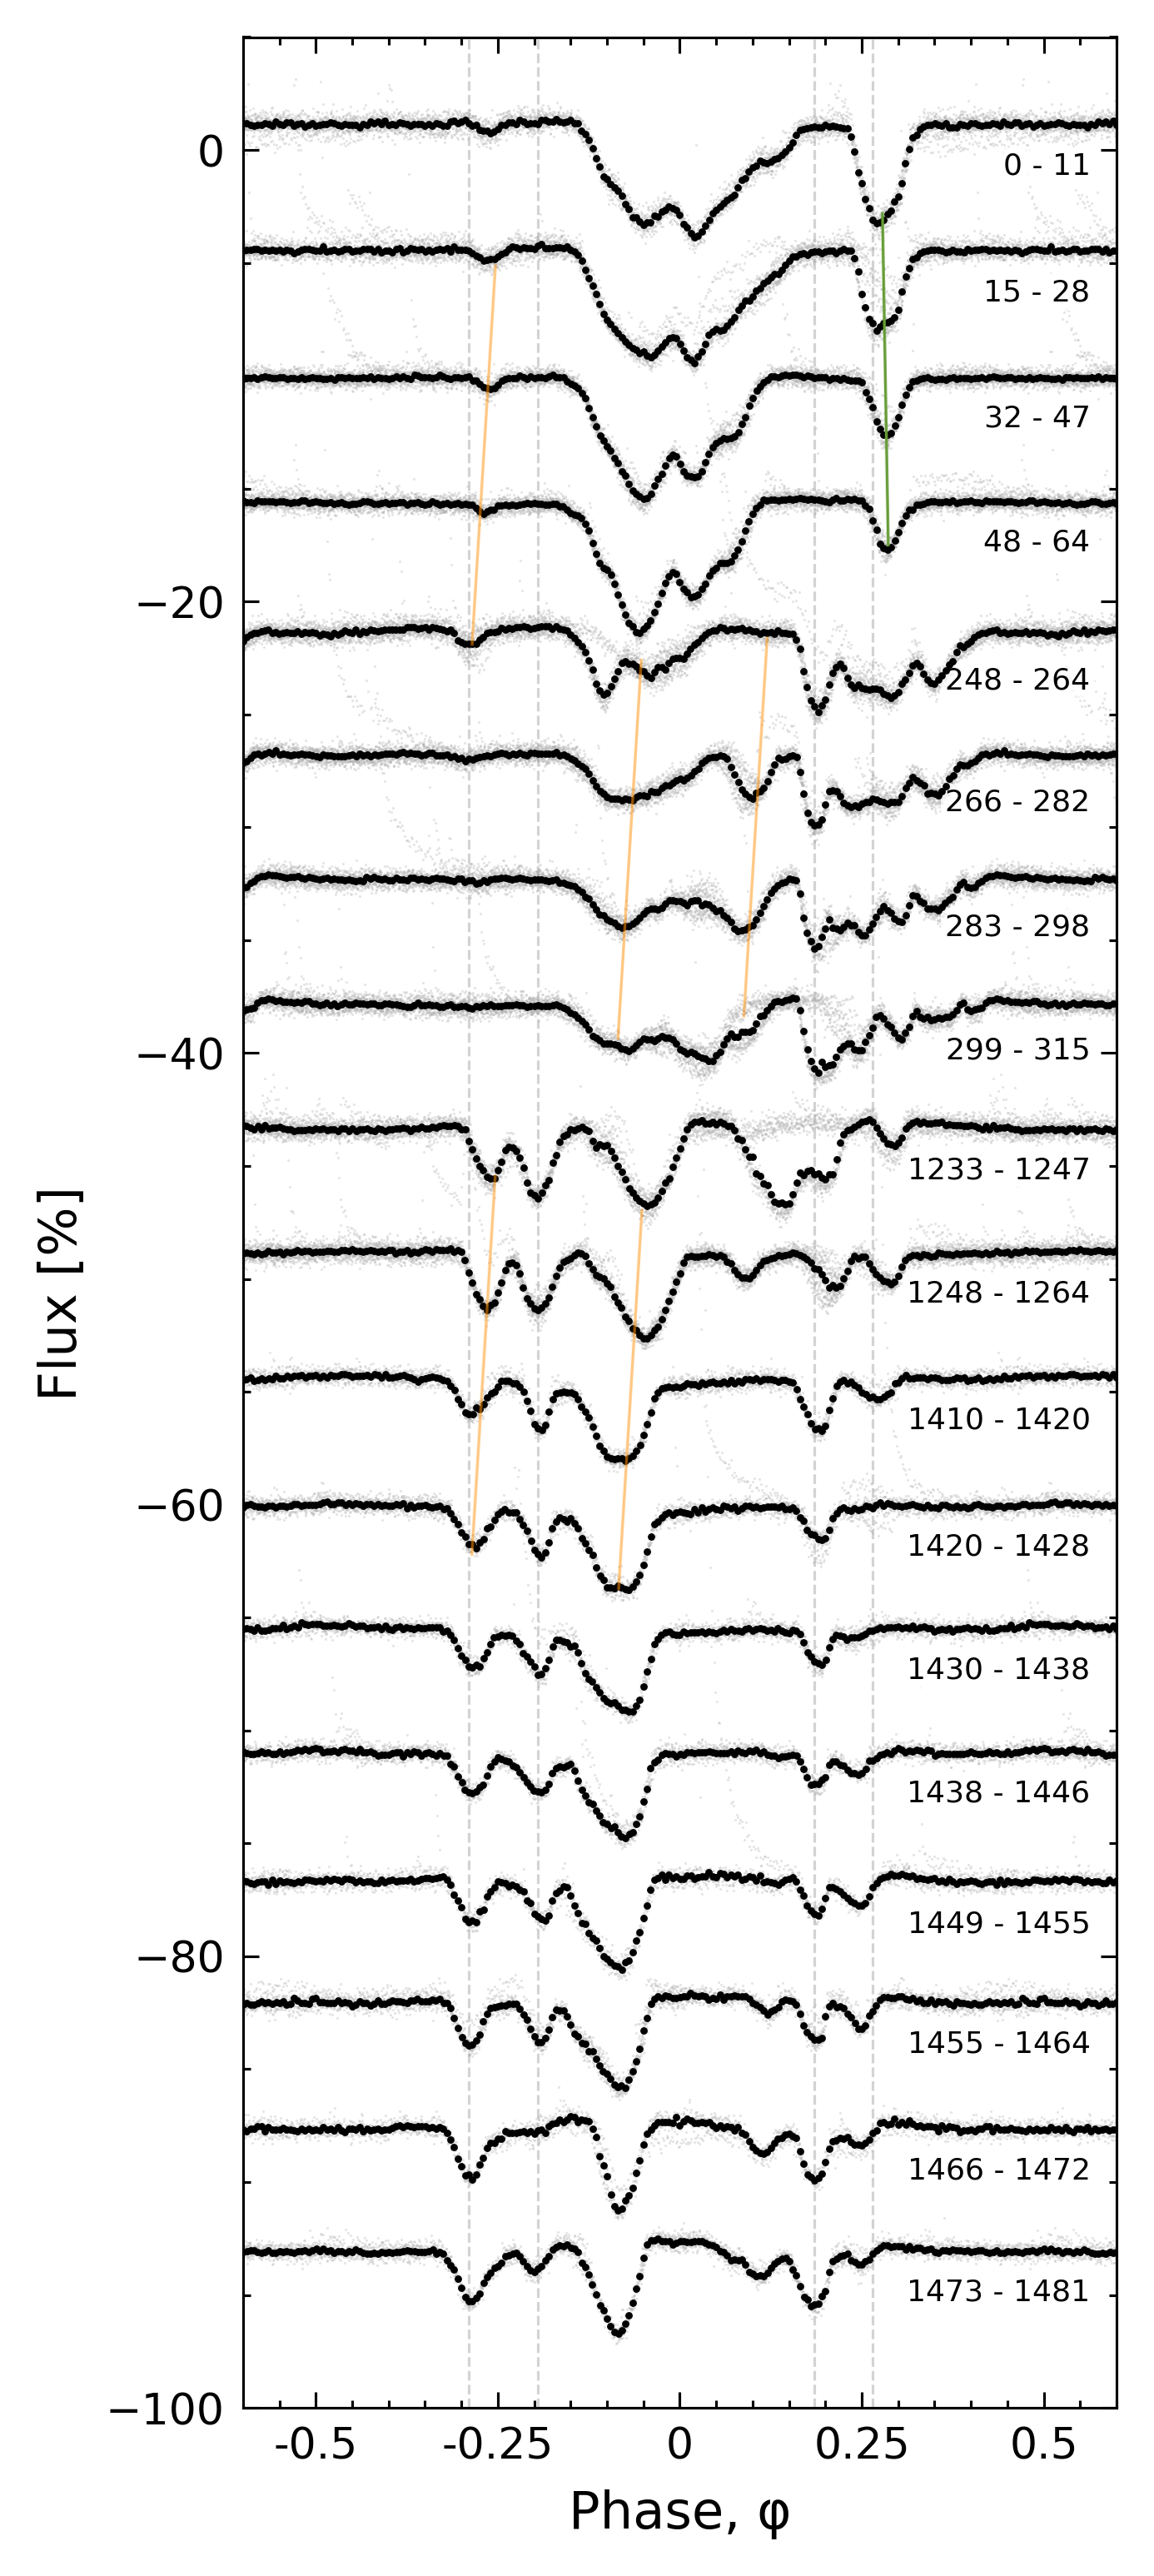
\includegraphics[width=0.45\textwidth]{ANNOTATED_resid_TIC_402980664_P18.5611_2min_phase_timegroups.png}
%	\end{center}
%	\vspace{-0.4cm}
%	\caption{
%		{\bf Alternative view of the evolution of LP 12-502}
%		(Figure~\ref{fig:lp}), arranged to emphasize changes in transit
%		times.  There are 200 binned black points per $P$=18.5611\,hr cycle; a two-harmonic
%		sinusoid has been subtracted from the PDC\_SAP light curve.
%		Vertical gray lines are underplotted to help guide the eye to instances
%		in which preferred dip phases synchronize over long baselines.
%		The orange and green lines guide the eye to where dips
%		change the positions of their local minima; orange
%		lines have periods slightly less than $P$, the green line has
%		a period greater than $P$.
%	}
%	\label{fig:lp2}
%\end{figure*}


\begin{figure*}[!t]
	\begin{center}
		\subfloat{
			\includegraphics[width=0.46\textwidth]{f7a.pdf}
			\includegraphics[width=0.46\textwidth]{f7b.pdf}
		}
		\vspace{-0.2cm}
		
		\subfloat{
			\includegraphics[width=0.46\textwidth]{f7d.pdf}
			\includegraphics[width=0.46\textwidth]{f7c.pdf}
		}
	\end{center}
	\vspace{-0.4cm}
	\caption{
    {\bf River plots of the LP 12-502 light curve}, showing (clockwise
    from top-left) Sectors 18-19, 25-26, 53, and 58-59.  A
    two-harmonic sinusoid has been subtracted to highlight the sharp
    dips.  
    A fixed period and phase are adopted for all sectors; the dips
    across all observations are bounded by $\phi \in [-0.35,0.35]$.
    In Sectors 25-26 (cycles 248-315), periods are visible at
    the fundamental period of 18.5611\,hr, as well as at faster
    ($\phi$$\approx$0-0.07) and slower ($\phi$$\approx$0.25-0.27)
    relative periods based on the presence of blue dips with distinct
    slopes.  Multiple simultaneous periods are also visible in Sector
    53 (cycles 1234-1263) and Sectors 58-59 (cycles 1411-1479).  White
    chunks denote missing data.
    The state changes noted in red in Figure~\ref{fig:lplc} occur in
    cycles 261, 309, and 1241.
	}
	\label{fig:lpriver0}
\end{figure*}


\subsection{Evolution over consecutive sectors, \& LP 12-502}

A few of our complex rotators were near the TESS continuous viewing
zones (Figure~\ref{fig:catalogscatter}, top right).  Out of this
already small sample, LP 12-502 (TIC 402980664; $d$=21\,pc, $J$=9.4,
$T$=11.1) stood out due to the quality and content of its data.  We
discuss another interesting source, TIC~300651846, in
Appendix~\ref{app:tic3006}.  In this section, we describe the LP
12-502 observations and the possible implications.


\subsubsection{LP 12-502 observations}
\label{subsec:lpobservations}

Whenever LP 12-502 was located within a TESS sector, it was observed
at 120-second cadence.  Figure~\ref{fig:lplc} shows all the available
data, from Sectors 18, 19, 25, 26, 53, 58, and 59. Vertical offsets
were applied to separate the data from different spacecraft orbit
numbers; there are always two orbits per sector.  We binned the light
curve to 15-minute intervals to facilitate visual inspection.  Points
more than 2.5$\sigma$ above the median are drawn in gray, to prevent
outliers from seizing attention.  Data gaps are not connected by lines
(a common source of confusion in light curve visualization).
Figure~\ref{fig:lp} shows the same data after phase-folding each TESS
spacecraft orbit, assuming $P$=18.5611\,hr and a fixed reference epoch
of BTJD=1791.5367.  Finally, Figure~\ref{fig:lpriver0} shows ``river
plots'' of the same data, split into similar intervals: the Sector
18-19 data, 25-26 data, 53 data, and 58-59 data.  The river plots are
subject to one additional processing step: we fitted and subtracted a
maximum-likelihood two-harmonic sinusoid independently from the Sector
18-19 data, 25-26 data, and 53, 58, and 59 data in order to accentuate
changes in the dip timing and structure.

The average period, determined by measuring the PDM peak period over
each sector independently, was $\langle P \rangle = 18.5560$\,hr.  The
range between the maximum and minimum sector-specific periods was
measured to be about one minute.   However, a period shift of
$\pm$1\,minute leads to large phase drifts over the entire timespan of
observations.  One minute is $\approx$1/1000$^{\rm th}$ of a period,
and we have observed 1500 cycles.  By folding with a fine grid of
trial periods, we found that the choice $P=18.5611 \pm 0.0001$ causes
more of the features in the LP 12-502 light curve to maintain constant
phases over the entire dataset.

We now attempt to describe the complex morphology of the light curve
and its evolution.  For the first 64 cycles, the star shows four
obvious local minima.  We dub these dips $\{ 1, 2, 3, 4 \}$ at phases
$\{ -0.28, -0.08, 0, 0.25 \}$, respectively.  Dips 2 and 3 are part of
the same ``global'' minimum, which otherwise resembles a long eclipse.
Over cycles 0-64, the depth of dips 1 and 3 remain roughly fixed.  Dip
4 decreases in depth by about 2\%, and dip 2 increases in depth by
about the same amount (see Figure~\ref{fig:lp}).  A subtle fifth dip
may also be present at phase +0.08, at the end of the global minimum
that includes dips 2 and 3.

There is then a 6-month (184-cycle) gap to Cycles 248-315, which show
two highly structured dip complexes, plus a small leading dip.  The
leading dip has the same phase (relative to minimum light) as in
cycles 0-64, and therefore seems likely to be due to the same
structure.  Along a similar line of logic, it seems plausible that the
first ``dip complex'' during cycles 248-264 represents an evolution
and reduction in amplitude of dips 2 and 3 that were seen during
cycles 0-64.  During cycles 266-310, an additional local minimum
develops between the two complexes; this feature is best visualized on
the river plots (Figure~\ref{fig:lpriver0}), where it is seen to have
a shorter period than the other dips (as described below).

The second dip complex during cycles 248-315 shows the most
substructure.  During e.g.~cycles 283-298, this single complex shows
six local minima.  The first and deepest dip is sharp: it shows a flux
excursion of 3.5\% over about 22 minutes (0.02\,$P$), which is the
steepest slope exhibited anywhere in the LP~12-502 dataset.  After the
sharp dip, there is a roughly exponential return to the baseline flux
spanning about a quarter of a period, punctuated by coherent local
minima and maxima that the river plot (Figure~\ref{fig:lpriver0})
reveals to have slightly longer periods than the sharp dip.  The sharp
leading dip remains roughly constant in amplitude until a sudden
``state change'' at BTJD 2030.7 (cycle 309) that occurred at the same
time as a flare, and left the trailing dips seemingly unaffected.
This apparent state change, and two others, are marked with red lines
in Figure~\ref{fig:lplc}.

The behavior during Sectors 53--58 (cycles 1233-1481) is comparatively tame; the light curve shows
only four to six dips per cycle.  Some dips remain stable in depth and
duration over this five-month interval.  Other dips grow, like the one
at $\phi = +0.06$ between cycles 1499 and 1481.  Other dips, such as
the one at $\phi = +0.12$ in cycles 1233-1264, disappear entirely.
The most dramatic state change occurs during cycle 1241, when a large
dip switches from a depth of 3\% and a duration of 3 hours to a depth
of 0.3\% and a duration of 1 hour.


\subsubsection{Lessons from LP 12-502}
\label{subsec:lplessons}

{\sc State-changes reveal dip independence}---The state-changes seen
in cycles 1233-1247 and 299-315 confirm that dips can disappear in
less than one cycle. While such behavior was also noted by
\cite{2017AJ....153..152S}, the data presented here show further that
the dips can be {\it independent} and {\it additive}.  For example,
throughout cycles 1233-1264, there are three sharp dips between phases
of 0 and 0.3 with different amplitudes but similar slopes.  During the
transition, the leading dip nearly disappeared while the other two
dips hardly changed; compare the centermost two panels of
Figure~\ref{fig:lp}.  Evidently, the material or process responsible
for one dip can vary independently of the materials or processes
responsible for other dips.  The state changes during cycles 248-264
and 299-315 support the same conclusion, while also hinting that the
{\it leading} dip of a complex is most prone to disappearing, leaving
the trailing dips unchanged in its wake.


{\sc Slow growth; rapid death}---LP 12-502 shows at least three
instances in which dips switch off over less than one cycle; we did
not see any such instances of dips switching on.  Dip growth seems to
happen more slowly.  For instance, the dip at phase 0-0.1 between
cycles 258-290 begins to become detectable during cycle 258, and
growths in depth by about 2\% over the next eight cycles.  The
evolution of this particular dip is most clear in the river plots.
The evolution of the dip group at phases 0.1-0.3 during cycles
1410-1481 is another example of this slow mode of dip growth.

% 16 px vs 310 px for a full phase
% Based on our SED fitting $R_\star=0.369\,R_\odot$ star, and from the
% isochrone mass, $M_\star=0.215\,M_\odot$ 

{\sc Dip durations}---The shortest dip duration for any of the
individual LP 12-502 dips seems to be $\approx$0.06\,$P$ $\approx$
1.08\,hr.  This is very similar to the characteristic timescale of a
transiting small body at the corotation radius,
\begin{equation}
T_{\rm dur} \equiv R_\star P_{\rm rot} / (\pi a) = 1.02\pm 0.10\,{\rm hr},
\end{equation}
where we have inserted the stellar radius and mass derived in
Section~\ref{subsec:starprops}.  Thus, the shortest-duration dips
could be produced by transits of bodies or distributions of material
that are smaller than the star.  The corotation radius corresponds to
$a/R_\star \approx 5.8$, i.e., the transit of a body at the corotation
radius has a duration about six times shorter than a feature on the
stellar photosphere that is carried across the visible hemisphere by
rotation.  On the other hand, some dip durations are sufficiently long
that an explanation involving transits would require structures that
are larger than the star along the direction of orbital motion.

{\sc Dip periods}---Most of the LP 12-502 dips repeat with a period of
$P=18.5611 \pm 0.0001$\,hr.  However the river plots
(Figure~\ref{fig:lpriver0}) reveal that a few dips have detectably
distinct periods.  For instance, in sectors 25-26, the dip that
develops around cycle 262 has a period shorter than the mean period by
$\approx$0.1\%, and some of the trailing local minima in the main dip
complex have periods slower than the mean period by $\approx$0.04\%.
In addition to the fundamental period, we were able to identify at
least four distinct periods shown by specific dips over the full
Sectors 18-59 dataset: 18.5683, 18.5672, 18.5473, and 18.5145\,hr,
with a measurement uncertainty of $\approx$0.0002\,hr. Possibly, the
different periods belong to clumps of dust or prominences of gas at
slightly different orbital distances surrounding the corotation
radius.



\section{Discussion}
\label{sec:discussion}


\subsection{Typical and extreme CRs}
\label{subsec:extreme}

Referring back to Figure~\ref{fig:catalogscatter}, which compares the
properties of CRs with those of the search sample (top panels) and the
Pleiades \citep{2016AJ....152..114R}, we see that the typical CR
masses span 0.1-0.4\,$M_\odot$, and the typical ages span 2-150\,Myr.
This mass and age range includes both fully convective stars and stars
with a combination of radiative cores and convective envelopes, with
the dividing line at around $M_\star = 0.25\,M_\odot$
\citep{2018A&A...619A.177B}.  We found no obvious differences in light
curve morphology between CRs above and below the boundary of
0.25\,$M_\odot$.  In terms of their rotation rates relative to the
Pleiades, the CRs are among the more rapidly rotating half of M
dwarfs. 

The closest CR in our catalog is DG~CVn (TIC~368129164; $d$$=$18\,pc),
a member of AB Dor.  To our knowledge, this star had not previously
been recognized as a CR.  The three brightest CRs are DG~CVn
($T$=9.3), TIC~405754448 ($T$=9.6), and TIC~167664935 ($T$=10.3).  The
shortest period, 3.64\,hr, belongs to TIC~201789285.  The longest
period, 37.9\,hr, belongs to TIC~405910546.  If the latter source
turns out to be an eclipsing binary, the longest-period CR in the
catalog would be TIC~193831684 (31.0\,hr).  By definition, we required
the periods to be below 48\,hr.

The lowest mass ($\approx$$0.12$\,$M_\odot$) belongs to TIC~267953787.
The catalog contains a few other stars with similar mass.  We cannot
rule out the possibility that CRs exist with even lower masses, given
the small number of such low-mass stars in our target sample.  Perhaps
even brown dwarfs can be CRs, although it might be difficult to
distinguish the type of variability we associate with CRs from the
usual variability of brown dwarfs caused by clouds and latitudinal
bands \citep[e.g.][]{2021ApJ...906...64A,2022ApJ...924...68V}.



\subsection{CRs and binarity}
\label{subsec:discbinary}

\subsubsection{Binary statistics}

In Section~\ref{subsec:binarity}, we found that a significant fraction
of the CRs show indications of unresolved binarity.  Excess noise
above the Gaia single-source astrometric model is common
(\ngoodhighruwe/\ngoods\ high-quality CRs with RUWE$_{\rm DR3}$$>$2),
as is the presence of multiple periods in the TESS light curves
(\ngoodmultperiodflag/\ngoods).  Elevated astrometric noise is almost
always accompanied by multiple detectable TESS periods
(\ngoodruweandmultperiod/\ngoodhighruwe\ high-quality CRs).  The
latter observation corroborates the claim that most sources with
RUWE$_{\rm DR3}$$>$2 are binaries with projected apparent separations
below 1$''$, and projected physical separations $\lesssim$50\,AU.

One possible relation between binarity and CRs is that the presence of
an intermediate-separation binary could cause early disk dispersal,
freeing the star to contract.  The CR phenomenon seems to require
rapid rotation; thus if binary systems tend to produce more rapidly
rotating stars, we would expect a sample of CRs to have a larger
binary fraction than the field.  We do not see clear evidence for such
an effect.  The multiplicity rate of M dwarfs near the Sun is
26.8$\pm$1.4\% \citep{2019AJ....157..216W}.  Based on the same study,
the peak of the separation distribution decreases from $\approx$49\,AU
for $0.30$-$0.60$\,$M_\odot$ stars, to $\approx$11\,AU for
$0.15$-$0.30$\,$M_\odot$ M dwarfs.  The multiplicity fraction in our
CR sample seems approximately consistent with this field fraction.



\subsubsection{Do K dwarf CRs exist?}
\label{subsec:massive}

To date, the only stars reported to show the CR phenomenon are M
dwarfs, with typical stellar masses $\lesssim$0.3\,$M_\odot$
\citep{2017AJ....153..152S,2022AJ....163..144G}.  However the two most
massive CRs in our sample, TIC~405754448 and TIC~405910546, were
assigned masses of $\approx$0.82\,$M_\odot$ and
$\approx$0.60\,$M_\odot$ respectively.  The next-highest masses in our
sample are $\approx$0.40\,$M_\odot$.

These stars' locations in color--absolute magnitude diagrams and
their probable membership in Lower Centaurus Crux both support the
conclusion that they have relatively high masses.
However in detail, both are subject to ambiguities
in interpretation.  The TIC~405910546 light curve has a unique shape,
suggestive of an eclipsing binary.  Independently, TIC~405910546 was
one of only \nrvscatterflag\ CRs flagged with a Gaia DR3 radial
velocity scatter exceeding 20\,\kms.  Combined, these factors suggest
that TIC~405910546 could be a pre-main-sequence eclipsing binary; it
should be studied further to clarify this classification.

For the other object, TIC~405754448, the evidence for binarity is
stronger.  The RUWE$_{\rm DR3}$ statistic is 6.8, and the raw light
curves in Sectors 11, 37, and 38 show both the CR signal with period
12.9\,hr and amplitude $\approx$1\% and an additional sinusoidal
signal with a period $\approx$6.5\,days and amplitude $\approx$0.3\%,
likely from a second star.  If TIC~405754448 is a K+M binary, then the
flux ratio between the primary and secondary would be expected to be
$\approx$10:1.  Thus, if the K star were the source of the CR signal,
its intrinsic variability amplitude would be $\approx$1\%, while if
the M star were responsible its intrinsic variability amplitude would
be $\approx$10\%.

In short, these two objects suggest that the CR phenomenon may extend
up in mass to pre-main-sequence K dwarfs, but more data are needed to
substantiate this claim.


\subsubsection{An astrophysical CR false positive: TIC~435903839}

We originally classified TIC~435903839, with RUWE$_{\rm DR3}$=17.7, as
an ``ambiguous'' CR with a 10.8\,hr period, because this period
minimized the dispersion in the phase-folded light curve.  More
careful inspection revealed an impostor:
this source is a photometric blend of two ordinary rotating stars with
$P_0$=3.60\,hr, and $P_1$=5.41\,hr, giving a beat period $(P_0^{-1} -
P_1^{-1})^{-1}$ of 10.8\,hr.  This is a novel false positive scenario
for CRs: two rapidly-rotating stars with near-integer ratios of
rotation periods.  The beat between the two rotation signals produces
the apparent CR signal.  Such false positives can be excluded through
careful accounting of all peaks in a periodogram.  For instance,
TIC~435903839 shows a peak at 16.27\,hr, which is not an integer
multiple of the dispersion-minimizing 10.82\,hr period.

\subsubsection{Multiple CRs in the same system: TIC~425937691 and TIC~142173958}

TIC~142173958 and TIC~425937691 both show evidence for two separate CR
signals in their TESS light curves.  For TIC~142173958, the signals
have periods of 11.76\,hr and 12.84\,hr.  For TIC~425937691, the two
periods are 4.82\,hr and 3.22\,hr, near the 3:2 commensurability.
Given that both sources have two photometric signals and elevated
RUWEs, each source is probably an unresolved binary consisting of two
CRs.

Recent work has shown that the orbits of binaries closer than
$\lesssim$700 AU tend to be aligned with their planetary systems
\citep[e.g.][]{2022AJ....163..207C}.  If we assume that observing CR
variability requires high inclinations relative to the line of sight,
and that the inclinations in binaries are correlated, then we would
expect the detection of one CR in a binary system to raise the
probability that the other star is a CR.  The limitations of the
current catalog prevent further exploration of this issue, but it
might be interesting for future study.  Even if this scenario is
correct, it would not provide an immediate explanation for the
near-commensurability of the two periods of TIC~425937691 (the ratio
is within 1\% of 3:2).



\subsection{Transience \& special phases of CR dips}

While CR periods appear to remain constant to within measurement
precision over thousands of cycles, the light curve shapes evolve over
typical timescales of 10 to 1{,}000 cycles (e.g.
Figures~\ref{fig:evoln} and~\ref{fig:lpriver0}).  The CRs are
therefore quasiperiodic, with a characteristic dip longevity of
$\approx$100 cycles.  While this observation is consistent with the
analyses by \citet{2022AJ....163..144G} and
\citet{2023ApJ...945..114P}, it marks a qualitative departure from the
``persistent'' {\it vs.} ``transient'' flux dip distinction described
by \citet{2017AJ....153..152S}, since all CR dips seem to be transient
over timescales of more than 1{,}000 cycles (Figure~\ref{fig:evoln}).

One peculiarity of CR evolution however is that the dips do not
explore all phase angles with equal weight.  LP 12-502, and other CRs,
have preferred phases lasting for at least two years.  For LP 12-502,
all of the dips happen over phases corresponding to only two thirds of
the period (Figures~\ref{fig:lp} and~\ref{fig:lpriver0}).  The
remaining third seems to be ``out of limits'' for dips over the
timespan of observations.  This could be evidence that the stellar
magnetic field is not azimuthally symmetric.  Alternatively, the
source of the material (e.g. a planetesimal swarm) might be
distributed over an arc rather than occurring randomly around the
entire orbit.  



\subsection{Dip asymmetries and dust geometries}

The asymmetry of a dip around the time of minimum light might be
caused by the variation in optical depth of the occulting material as
a function of orbital phase angle.  Sharp leading edges with trailing
exponential egresses, for instance, have been previously seen for
transiting exocomets and disintegrating rocky bodies
\citep[e.g.][]{2012ApJ...752....1R,2012A&A...545L...5B,2015Natur.526..546V,2019A&A...625L..13Z}.

Examining Figure~\ref{fig:cqvs}, it is clear that CR dips can be
asymmetric but it is not obvious whether there is a preference for
sharper ingresses or sharper egresses.  In some cases (e.g.
TIC~425933644), the flux variations do not resemble isolated dips,
making the meaning of ``ingress'' and ``egress'' unclear.  In other
cases, such as Sector~36 of TIC~89463560, there is a sharp drop with
an exponential return to the baseline flux, resembling the signatures
of exocomet \citep[e.g.][]{2018MNRAS.474.1453R,2019A&A...625L..13Z},
or the outflowing exospheres of certain transiting planets
\citep[e.g.][]{2019ApJ...873...89M,2022ApJ...926..226M}.



\subsection{Dust vs. gas}

Both the dust clump and the gas prominence scenario invoke clumps
of material at the corotation radius;
the main property that we believe distinguishes the two ideas is 
the composition of the material.

\subsubsection{What is a prominence?}
The prominence idea is based on an analogy with quiescent
prominences/filaments in the solar corona that last as long as a few
weeks \citep[see][]{2015ASSL..415.....V}.  In the context of the Sun,
a prominence is a clump of cold, partially ionized hydrogen viewed in
emission against the dark backdrop of space.  A filament is the same
clump of plasma, but viewed in absorption against the solar disk.  In
an extrasolar context, spectroscopic detections of transient Balmer-
and resonance-line absorption seen for stars such as AB~Dor and
Speedy~Mic
\citep[e.g.][]{1989MNRAS.238..657C,1993MNRAS.262..369J,2006MNRAS.365..530D,2016MNRAS.463..965L}
have been interpreted as prominences that scatter a star's
chromospheric emission \citep[see][]{1989MNRAS.238..657C}.  The
short-term mechanical stability of such gas configurations is
theoretically plausible for rapidly rotating stars
\citep{2000MNRAS.316..647F,2022MNRAS.514.5465W}.   To our best
knowledge, this class of spectroscopic observation also has no viable
alternative explanations.

We performed a simple visual examination of the TESS light curves for
five prominence-hosting systems studied by
\citet{2019MNRAS.482.2853J}--AB~Dor, Speedy~Mic, LQ Lup, HK Aqr, and
V374 Peg--and detected no CR behavior.  Assuming that
spectroscopically observable prominence systems do not turn off, this would
imply that they are not always accompanied by photometric CR-like
dips: a link between the spectroscopic prominences
that may exist around rapidly rotating low-mass stars and the CR
phenomenon has yet to be made.  


\subsubsection{What is the microphysical source of opacity?}

CRs show broadband flux variations that can be 1-2$\times$ deeper in
the blue than in the red
\citep{2017PASJ...69L...2O,2020AJ....160...86B,2022AJ....163..144G,2023MNRAS.518.2921K}.
Dust can naturally explain this chromaticity, since it has a larger
absorption cross-section in the blue than the red
\citep[e.g.][]{1989ApJ...345..245C}.  Gas might also explain the observed
chromaticities \citep{1992oasp.book.....G}.  While bound-bound
absorption can be excluded, since it provides opacity only at narrow
resonant lines, the (neutral) hydrogen opacity due to bound-free
absorption is ``jagged'' \citep[see][Figure 8.5 and
Eq.~8.8]{1992oasp.book.....G}, such that at temperatures of
$\approx$3{,}000\,K to $\approx$10{,}000\,K the opacity can be larger
at blue wavelengths than at red wavelengths.  Bound-free absorption of
${\rm H}^{-}$ is often important at such temperatures, but this
opacity source is stronger in the red than the blue, the opposite of
what is required to produce deeper dips in the blue than in the red.
Likewise, Thomson scattering is too gray to be the dominant opacity
source.

An instructive point of comparison is the rapidly rotating magnetic B
star, $\sigma$~Ori~E, which shows dips that are deeper in the blue
than in the red \citep{1977ApJ...216L..31H}.  Photometric and
spectroscopic observations of this star have been understood in terms
of a warped torus of corotating circumstellar material
\citep{1978ApJ...224L...5L,1985Ap&SS.116..285N,2005ApJ...630L..81T}.
The circumstellar material is unlikely to be dust, which would
sublimate quickly at the distance of the torus from the
star.\footnote{\citet{2019ApJ...876..127Z} explored the sublimation
timescales for a canonical CR with $M_\star=0.2\,M_\odot$,
$R_\star=0.3\,R_\odot$, and $T_{\rm eff}=3200\,{\rm K}$.  They found
that non-shielded, generic silicate dust mixture \citep{1985ApJS...57..587D} with a
single size of 0.1\,$\mu$m reached the $\approx$1500\,K sublimination
temperature at $\approx$3\,$R_\star$.  This suggests that dust
sublimation could be an important effect even for CRs. }  The opacity
source for $\sigma$~Ori~E and its analogs is instead thought to be
bound-free absorption by neutral hydrogen \citep{1985Ap&SS.116..285N},
although to our best knowledge direct evidence for this conclusion has
yet to be acquired.  Separate and smaller-amplitude continuum flux
brightenings in $\sigma$~Ori~E may also come from electrons scattering
photospheric light toward the observer when the clouds are not
transiting \citep{2022MNRAS.511.4815B}.

Given these complexities, it seems important for a future theoretical
study to be conducted to determine to what degree the observed
chromaticities in CRs match, or do not match, expectations from
radiative transfer.  This issue has a key ability to resolve the
question of whether the CRs are explained by dust or by gas, which has
bearing on whether the material producing the dips is coming from the
star, or whether it is a byproduct of the protoplanetary disk.



\subsubsection{The lifetime constraint}

The observed lifetime of the CR phenomenon could provide another way
to discern between the gas and dust clump scenarios.  Based on the
available statistics from e.g.  \citet{2022AJ....164...80R} and
references therein, it seems plausible that CR occurrence decreases
with stellar age from $\approx$3\% at 10\,Myr (Sco-Cen),
to $\approx$1\% at 100\,Myr (Pleiades),
down to 0\% by the $\approx$700\,Myr
age of Praesepe.  This is odd in the context of the prominence
scenario, because pre-main-sequence M dwarfs spin up over the first
100\,Myr; prominences might therefore even be expected to be {\it
more} common at 100\,Myr than at 10\,Myr, under the assumption that the
production of prominences depends only on the stellar rotation rate. 
The dust clump scenario would hold a natural explanation: the lower occurrence of CRs around older stars would
simply reflect a finite supply of dust.
One possible complication however is that the magnetic field topology
of rapidly rotating M dwarfs may depend on factors other than the
rotation rate (e.g. the age), which might affect the production of prominences.


\subsection{Planets or planetesimal swarms near corotation?}

Close-in planets are common around M dwarfs; studies from Kepler have
shown that early M dwarfs have $\approx$0.1 planets per star with
sizes between 1-4\,$R_\oplus$ and orbital periods within 3 days
\citep{2015ApJ...807...45D}.  The frequency of planets per star
increases to $\approx$0.7 when considering periods as long as
10\,days.  Extrapolating to all small (0.1-4\,$R_\oplus$) planets within
10 days, it is reasonable to expect
nearly all M dwarfs to have at least one planet.

In the context of disk-driven planet migration, the stopping location
for the innermost planet is set by the location of the protoplanetary
disk's truncation radius \citep{2018haex.bookE.142I}.  The 
truncation radius is traditionally calculated by equating the magnetic
pressure from the stellar magnetosphere with the ram pressure of the
inflowing gas.  As it happens, the truncation radius is close to the
corotation radius for low accretion rates
\citep{2016ARA&A..54..135H,2022MNRAS.510.5246L}.  These considerations
invite us to imagine one or more planets migrating inward due to gas
drag, and arriving at $\approx$5-10 stellar
radii before the disk is depleted.

With this picture in mind, it is tempting to attribute features of the
CR light curves as transits of material ejected by planets or
planetesimals.  Young rocky bodies are expected to be hot, and they
might expel either gas or dust.  The Jupiter-Io
system \citep[e.g.][]{2004jpsm.book..537S} is analogous, in that a small rocky
body similarly feeds the construction of a plasma torus.  We emphasize
that while this type of configuration seems a priori plausible, no
direct evidence currently supports it.

The main logical function of the planetesimals would be to serve as a
source for the occulting gas or dust; they would not necessarily need
to explain the observed phases of the observed dips.  The azimuthal
angle of the eventual entrainment would be entirely determined by the
stellar magnetic field.  In this scenario, the obscuring material
would inspiral from one or more rocky bodies well beyond the
corotation radius.  The planetesimals themselves would not necessarily
need to transit.  However if they did, they would need to be $\lesssim
1$\,$R_\oplus$ based on their non-detections in the TESS data.
Possibly analogous systems include K2-22 \citep{2015ApJ...812..112S}
and KOI-2700 \citep{2014ApJ...784...40R}, though the obscuring
material in the CRs would need to be observed much further from the
emitting planet than for those two examples.  

A more restrictive variant of the planetesimal scenario would be to
posit that the obscuring material remains close to the launching body,
similar to comets, or to the aforementioned K2-22 and KOI-2700
systems.  If so, then the planetesimals would need to be at the
corotation radius.  One prediction would therefore be that certain
orbital phases would produce recurrent dips when observed over
sufficiently long baselines, because the launching planetesimal would
be massive enough to remain in orbit, while stochastically ejecting
material.  For most CRs (Figure~\ref{fig:evoln}), the data seem to be
in tension with this expectation because the relative spacing between
dips is almost never conserved.  With that said, certain sources do
seem to exhibit ``special phases'', including LP 12-502
(TIC~402980664), DG~CVn (TIC~368129164), TIC~193831684, and
TIC~146539195.  One possible explanation for this might be if
obscuring material is remaining close to its launching body, or
bodies.  An alternative explanation could be that the stellar magnetic
field configurations responsible for confining said material are
stable over the existing two-year baseline.



\subsection{From dippers to debris disks}
\label{subsec:discdippers}

About one in three young stars with infrared-detected inner dusty
disks show quasiperiodic or stochastic dimming over timescales of
roughly one day \citep[e.g.][]{2010A&A...519A..88A}.  The dimming
amplitudes can reach a few tenths of the stellar brightness, and dips
with identical depths and phases rarely recur.  These ``dipper'' stars
are probably explained by occulting circumstellar dust in the inner
disk
\citep[e.g.][]{2014AJ....147...82C,2016ApJ...816...69A,2021ApJ...908...16R,2022ApJS..263...14C}.
While the phenomenon can persist beyond $\approx$10\,Myr
\citep{2019MNRAS.488.4465G,2022MNRAS.514.1386G}, in all such cases it
seems to be associated with the presence of infrared excesses.
Phenomenologically, dippers are different from CRs in that their dips
are usually deeper, less periodic, and more variable in depth over
timescales of only one or a few cycles.  Dipper stars also tend to be
younger, since they tend to be classical T Tauri stars with infrared
excesses.

In identifying the two candidate CRs with outlying SEDs
(TICs~193136669 and TIC~57830249; Section~\ref{subsec:irexcess}), we
were prompted to reconsider our light curve-based labeling, and
ultimately concluded that these sources are dippers.  This episode
suggests that there could be overlap between CRs and dippers.  Taking
TIC~57830249 as one example, the Sector~36 TESS data are suggestive of
a CR, with relatively periodic, sharp dips with depths of a few
percent.  The Sector~10 data are completely different, varying in
apparent flux by a factor of two, with no discernible periodicity at
all.  Perhaps this source becomes a ``dipper'' when an inflow of dust
reaches the inner disk wall, and is otherwise a ``CR'' when the inner
disk is starved of dust.

Although this outlier is intriguing, stars without infrared excessess
typically have more stable optical light curves than those with
infrared excesses.  While some dippers may evolve into CRs after the
disk is mostly gone, this would be generically expected based on the
population statistics: young stars become older.  There may be no
other causal connection between the two evolutionary stages.  With
that said, a common mystery between the CRs and dippers is how exactly
the {\it narrowness} of the dust-induced dimmings is produced.  It is
not unreasonable to imagine a similar mechanism operating for both
types of object, tied perhaps to a shared magnetic topology, or
perhaps to a preference for dust to inspiral to the star in clumped
structures.


%\subsection{Are half-cycles important?}
%
% NOTE to arxis readers: the answer was: "maybe in a few cases, but
% this manuscript was already too long!".
%
%The interval of half a cycle period could be significant in the
%context of CRs for two reasons.  The first is that for material on a
%circular orbit viewed edge-on, a half-cycle corresponds to the
%interval between transit and secondary eclipse.  The second is that
%the half-cycle also corresponds to the interval over which half of the
%star's surface is visible.  Of the CRs in Figures~\ref{fig:cqvs}
%and~\ref{fig:evoln}, a fraction that seems greater than random might
%exhibit a preference for showing dips or peaks that correspond to the
%half-cycle interval.
%
%One set of CRs shows ``CR behavior'' (some form of dip complex), but
%which only lasts for half of any given cycle.  TIC~206544316 (Sector
%2) is a canonical example; TIC~405910546 (Sector 38), TIC~167664935
%(Sector 38), TIC~146539195 (Sector 5), TIC~118449916 (Sector 44), and
%TIC~312410638 (Sector 38) seem to show the same tendency.
%
%An independent set of CRs exhibits small dips roughly half a cycle
%after large dips; it is tempting to label the small dips secondary
%eclipses.  Such sources include TIC~402980664 (Sector 25; relative to
%the sharpest, deepest minimum), TIC~89463560 (Sector 36),
%TIC~224283342 (Sector 2), and TIC~442571495 (Sector 12).  For the
%particular case of TIC~224283342, this observation, coupled with Gaia
%DR3 radial velocities suggesting a radial velocity scatter exceeding
%20\,\kms, suggests that the system could be a low-mass eclipsing
%binary transiting a giant polar spot, analogous to TOI-3884
%\citep{2022A&A...667L..11A}.
%
%In general however, it is challenging to interpret the significance of
%the potential ``half-period regularities'';  the CRs exhibit such a
%wide range of variability that for seemingly any regularity one might
%posit, it is easy to come up with counter-example objects which do not
%follow the trend.  In other words, these half-cycle CRs could simply
%be a product of the human tendency to pattern match.


\begin{figure}[!th]
	\begin{center}
		\centering
		\subfloat{
			\includegraphics[width=0.48\textwidth]{f9a.pdf}
		}
			
		\vspace{-0.35cm}
		\subfloat{
			\includegraphics[width=0.48\textwidth]{f9b.pdf}
		}

		\vspace{-0.35cm}
		\subfloat{
			\includegraphics[width=0.48\textwidth]{f9c.pdf}
		}

		\vspace{-0.1cm}
		\caption{
      {\bf The magnetic B star connection.}
      $\sigma$~Ori~E and HD~345439 (top row) are magnetic B stars with
      predominantly dipolar magnetic fields known to host
      circumstellar plasma tori.  HD~37776 and HD~64740 (middle row)
      are analogous magnetic B stars with field topologies dominated by
      high order multipoles.  The bottom row compares the latter
      systems against the ``best-matching'' CR light curves, selected
      by eye from Figure~\ref{fig:cqvs}.  CRs have light curves that
      are visually similar to the topologically complex magnetic B
      stars.  Stellar masses rounded to one significant figure are
      given in the lower right of each panel; the star, TESS sector,
      and period are listed in each subtitle.
		}
		\label{fig:bstar}
	\end{center}
\end{figure}


\subsection{Mass flux estimate}
\label{subsec:massflux}

Assuming for the moment that the obscuring material is dust, we can
estimate the mass of a transiting clump. First, we convert the transit
depth into an effective cloud radius, $R_{\rm cloud}$.  For most CRs
in Figure~\ref{fig:cqvs}, this yields $\approx$2-20\,$R_\oplus$.  A
minimum constraint on the number density of dust particles is obtained
by requiring the cloud to be optically thick.  For cases like LP
12-502, this is reasonable because the transit duration of the
shortest dips implies $R_{\rm cloud}\ll R_\star$.  Carrying out the
relevant calculation assuming the dust grains are 1\,$\mu$m in size,
\citet{2023MNRAS.518.4734S} reported minimum cloud masses of order
$10^{12}$\,kg (their Eq.~23), which scale linearly with both the
optical depth and dust grain radius.  This is comparable to a small
asteroid; the asteroid belt itself has a mass of order
$\approx$10$^{21}$\,kg \citep{2019Icar..319..812P}.  A similar
calculation that assumed occulting clupms of hydrogen, rather than
dust, derived gas prominence masses of at least $10^{14}$\,kg
\citep{1990MNRAS.247..415C}, about 100$\times$ larger than the lower
limit on the dust mass.

If the disappearance of a dip represents the permanent loss of the
obscuring material -- for example, if it is the result of a dust clump
being accreted or ejected -- then we can also estimate the rate at
which mass is flowing through the structures that lead to dips.  For
instance, LP~12-502 showed three ``state-switch'' events over the six
months of available TESS observations, during cycles 261, 309, and
1241 (Figure~\ref{fig:lpriver0}).  The other source for which we
performed a comparable analysis, TIC~300651846
(Appendix~\ref{app:tic3006}), showed two state-switches over 11
months.  In all such cases, at least one dip turned off.  For purposes
of estimation, we will take LP 12-502 as our prototype.  Assuming the
occulting material is dust, the corresponding $\dot{M} \equiv M\cdot
{\rm d}N/{\rm d}t$ time-averaged over six months is
$\approx$3$\times$$10^{-18} M_\odot\,{\rm yr}^{-1} \approx
1\times10^{-12} M_\oplus\,{\rm yr}^{-1}$.  Considered cumulatively
over the $\approx$$10^8$ years for which the CR phenomenon is
observed, this yields a cumulative moved dust mass of
$10^{-4}\,M_\oplus$, of order the Solar System's asteroid belt.  If
the occulting material is gas, the masses involved would be of order
100 times larger.  For cases in which we observe the {\it growth} of
dips, such as the Sector~29 data for TIC~224283342, or Sector~5 of
TIC~294328885, the dip depths typically increase by of order a few
percent over ten to twenty days.  This growth rate yields a mass flux
one order of magnitude larger than the earlier estimate.



\subsection{Strengthening the magnetic B star connection}

\citet{2017AJ....153..152S} previously noted a possible connection
between the CRs and rapidly rotating magnetic B stars such as
$\sigma$~Ori~E, which can have circumstellar gas clouds trapped in
corotation \citep{2005ApJ...630L..81T}.  The $\sigma$~Ori class is
distinct from Be-star decretion disks, which do not have any obvious
connection to the stellar magnetic field \citep{2013A&ARv..21...69R}.

An argument against the connection between CRs and the $\sigma$~Ori~E
analogs is that the light curve of $\sigma$~Ori~E is simpler than
those in Figure~\ref{fig:cqvs}, with only two broad local minima, and
one ``hump'' (Figure~\ref{fig:bstar}; see also
\citealt{2022ApJ...924L..10J}).  Within the model proposed by
\citeauthor{2005ApJ...630L..81T}, the simplicity of the light curve is
the result of a simple dipolar magnetic field, which is typical of
magnetic B stars \citep{2007A&A...475.1053A,2009ARA&A..47..333D}.  The
magnetic axis needs to be tilted relative to the stellar spin axis in
order to match the qualitative behavior of both the broadband light
curves, and the line-profile variations seen in hydrogen, helium, and
carbon \citep{2012MNRAS.419..959O}.

Two interesting and possibly telling exceptions to the rule that
magnetic B stars have simple light curves are HD~37776 and HD~64740.
Both stars are known from spectropolarimetry to have field geometries
dominated by high order multipoles \citep{2011ApJ...726...24K}.
And, recent TESS light curves of these two B stars appear surprisingly
similar to the CR light curves \citep{2020pase.conf...46M}.  The
middle row of Figure~\ref{fig:bstar} shows the phased TESS light
curves for these two stars, with by-eye best-matching CRs shown
underneath for comparison.  The number of dips per cycle, the shapes
of the dips, and the dip depths relative to the sinusoidal envelope
are all similar.  This connection suggests that the highly structured
light curves of both the M dwarfs and the B stars are associated with
(and perhaps caused by) strong non-dipolar magnetic fields.
Non-dipolar fields for M dwarfs are plausible, given that Zeeman
Doppler Imaging has revealed non-axisymmetric magnetic field patterns
for the few M dwarfs for which this technique is technically feasible
\citep[see][and references therein]{2021A&ARv..29....1K}.


The physical similarity between the B stars and the M dwarfs
presumably has its origin in the existence of a ``centrifugal
magnetosphere'' \citep[see][]{2013MNRAS.429..398P}.  In other words,
both classes of objects probably satisfy the condition $R_{\rm m} >
R_{\rm c}$, for $R_{\rm m}$ the magnetosphere radius (sometimes called
the Alfv\'en radius).  Provided that charged particles are confined to
move along magnetic field lines, stable points that balance the
centrifugal force and gravity can then exist at the corotation radius
\citep[e.g.][]{2005MNRAS.357..251T}.  In the converse ``dynamical''
case, when $R_{\rm m} < R_{\rm c}$, material interior to the
magnetospheric radius returns to the stellar surface over the
free-fall timescale.  A simple estimate assuming a dipole field with
$B_0\approx1\,{\rm kG}$ at the star's surface, a local plasma number
density $n\approx10^9\,{\rm cm^{-3}}$, and a plasma temperature
$10^6\,{\rm K}$ gives magnetospheric radii of order a few times the
corotation radii, $R_{\rm c}$.  This suggests that the existence of a
centrifugal magnetosphere is plausible for young, rapidly rotating M
dwarfs.

% NOTE to the arxiv crawlers:
%
% While there are some qualitative connections to Jupiter-Io, it's not
% perfect.  In that system, R_m>R_c...  But the plasma torus exists
% near Io's 42 hour orbit ...and is nonetheless STILL FORCED into
% corotation at a 10hr period (presumably by Jupiter's B-field).  This
% type of structure is very different, because here we actually see
% the plasma at the corotation radius itself!


\section{Conclusions}
\label{sec:conclusion}

In this work, we searched 120-second cadence TESS data collected from
2018 July to 2022 September for complex rotators (CRs).  The target
stars were \nstarssearched\ K and M dwarfs within 150\,pc.  The
selection function was $>$$80\%$ complete within 30\,pc, and $<$$10\%$
complete at distances exceeding 100\,pc.

In our target sample, we found \ngoods\ objects that showed complex
quasiperiodic behavior over at least one TESS sector.  These \ngoods\
bona fide CRs are listed in Table~\ref{tab:thetable}.  This table also
includes \nmaybes\ ambiguous CRs, whose designation is
less certain, and \ndebunked\ impostors.  We inferred ages for all but
two of the \nallcands\ objects based on memberships in young stellar assocations; we
also derived temperatures and radii using SED fitting, and 
inferred stellar masses by interpolating against stellar evolutionary
models.  We caution that our sample is far from being
volume-limited and is not even magnitude-limited:
the TESS 120-second stellar sample had a heterogeneous
selection function which may have been biased in favor of young stars
over field stars.  Previous work however has shown that $\approx$1-3\%
of M dwarfs younger than $\approx$100\,Myr show the CR phenomenon
\citep{2016AJ....152..114R,2022AJ....163..144G}.

Analyzing the TESS light curves and stellar properties of our CRs, we
draw the following conclusions.

\begin{enumerate}[leftmargin=*]
%
    \item The sharpest CR dips have durations of $\approx$0.05\,$P$
      and depths of $\approx$1-3\% (Figures~\ref{fig:cqvs}
      and~\ref{fig:evoln}).  Explaining dips this sharp requires
      material extrinsic to the stellar surface (see
      Section~\ref{sec:intro}).
%
    \item The shortest CR dips, also with durations of
      $\approx$0.05\,$P$, match the expected transit duration of a
      small body at the corotation radius, $T_{\rm dur} \equiv R_\star
      P_{\rm rot} / (\pi a)$ (see Section~\ref{subsec:lplessons}).
      Such dips may therefore be produced by transits of bodies or
      distributions of optically-thick material that are smaller than
      the star.
%
    \item Most CR dips have durations a few times longer than $T_{\rm
      dur}$ (Figure~\ref{fig:cqvs}).  The dips are often superposed
      on a quasi-sinusoidal signal that presumably comes from
      starspots and faculae that produce inhomogeneities in the
      longitudinal flux distribution across the stellar surface.  The
      only viable explanation currently known for the sharp dips being superposed on
      the quasi-sinusoidal signals is that concentrations (``clumps'')
      of circumstellar material are corotating with the star.
      Assuming that the longer dips have the same physical origin as
      the shortest dips, the transiting material must therefore also
      be capable of having effective sizes comparable to the star.
%
    \item The mean periods of CRs remain fixed to within a relative
      precision $\lesssim$0.1\% over the two-year ($\approx$1{,}000
      cycle) baseline of available observations.  The light curve
      shapes always evolve over this timescale
      (Figure~\ref{fig:evoln}).
%
    \item The dips in CR light curves can have slightly different
      periods.  LP 12-502, for instance, showed dips with four
      distinct periods within $\pm 0.3\%$ of its fundamental period,
      sometimes simultaneously, and each lasting for up to 50 cycles
      (Figure~\ref{fig:lpriver0}).
%
    \item The CR peaks and dips evolve over timescales that are both secular
      ($\approx$100\,cycles) and impulsive ($<$1 cycle).  Dip growth seems
      to happen over durations of at least ten cycles, and slow dip
      decay can also occur.  ``State-switches'' correspond to dips 
      collapsing instantaneously, and are almost always linked with
      observed optical flares.  Such switches are suggestive of
      magnetic reconnection opening the ``magnetic cage'' that traps
      the dust.
%
    \item The on-off duty cycle for CRs seems to be $\approx$$75$\%, based
      on the fraction of bona fide CRs that either turned on or turned
      off during TESS re-observations, two years after the initial
      observation (Figure~\ref{fig:evoln}).
%
    \item The CR phenomenon persists for $\gtrsim$150\,Myr, based on
      the existence of multiple CRs in AB Dor, the Pleiades, and
      Psc-Eri (Section~\ref{subsec:starprops}).  It may even extend to
      200\,Myr, based on the one CR we found in the Carina Near
      moving group (TIC~294328887; $\approx$200\,Myr).  However the
      lack of detected CRs in the Hyades and Praesepe suggests that
      the lifetime of the phenomenon is limited to the first few
      hundred million years.
%
    \item Most CRs are M dwarfs with masses
      0.1-0.5\,$M_\odot$.  Two sources, TIC~405754448 and
      TIC~405910546, have masses that appear to exceed the M dwarf
      limit.  However both are potentially binaries, and this may
      confuse our ability to accurate identify the source of the CR
      signal (Section~\ref{subsec:massive}).  We encourage additional
      scrutiny of these objects in future work.
%
    \item The closest CRs to the Sun are at distances of 15-20\,pc,
      and the brightest have $V$$\approx$12 ($J$$\approx$7.5).  We
      have found most of them in this work, since our CR sample was
      $\gtrsim$80\% complete within 30\,pc.  The lack of CRs in the
      volume-complete $<$15\,pc sample of 0.1-0.3\,$M_\odot$ stars
      analyzed by \citet{2021AJ....161...63W} is consistent with this
      estimate.  Expanding our analysis of the TESS data to the full
      frame images would yield a truly volume-limited selection
      function, and would expand the CR census by about a factor of
      two within 50\,pc, and by a factor of ten within 100\,pc.
%
    \item Surprising analogs to the CRs exist in two magnetic B stars
      with multipolar field topologies.  Since most magnetic B stars
      have dipolar magnetic fields, this suggests that the CR dips and
      warps are similarly being sculpted by the stellar magnetic
      fields, and that the magnetic fields themselves are potentially
      also multipolar.
%
    \item The rate of dip evolution can be used to place a
      model-dependent lower bound on how much material is either being
      accreted or ejected during the state changes
      (Section~\ref{subsec:massflux}).  Order of magnitude estimates
      require at least an asteroid belt's worth of dust
      ($10^{-4}$\,$M_\oplus$) over $10^8$ years, or at least
      $\approx$$10^{-2}$\,$M_\oplus$ if the occulting material is gas.
\end{enumerate}

While many questions remain, two in particular will be important for
clarifying what these objects might teach us in a broader
astrophysical context: {\it 1)} Is the eclipsing material responsible
for the phenomenon gas or dust?  {\it 2)} What sets the characteristic
clumping size for the circumstellar material?

The distinction between gas or dust is important because it will
clarify whether the CR phenomenon is intrinsic, so that material
comes from the star, or extrinsic, so that it is sourced through some
generic evolutionary phase of debris disks.  This knowledge would in
turn propagate to our understanding of whether the phenomenon is
primarily teaching us about dust production and processing in gas-poor
disks, or whether it is teaching us about the ability of cold gas to
remain stable in hot stellar coronae for long durations.
Observationally, acquisition of medium- or high-resolution time-series
spectra holds a good chance at resolving the gas vs.~dust question.
Given our observed $\approx$75\% on-off duty cycles, such data must be
acquired simultaneously with photometric time-series observations
(e.g. during TESS re-observation) in order for detections and
non-detections to be interpretable.

In both the gas and dust scenarios, CRs are preferentially viewed
edge-on.  This implies that after correcting for the line-of-sight
inclination, roughly one third of low mass stars \citep[those that
rotate rapidly enough;][]{2022AJ....163..144G} could trap circumstellar
material in the same way.  It also suggests that CRs may
preferentially show transiting planets at larger distances than the
corotating material, though this conclusion would be dependent on whether the
magnetic and stellar spin axes tend to be aligned.  Given these
points, observational follow-up work should include searching for
outer transiting planets, and measuring equatorial velocities in order
to test whether the stellar inclination angles are indeed
preferentially edge-on.  Any source of empirical information on the
stellar magnetic field, whether from the Zeeman effect
\citep[e.g.][]{2021A&ARv..29....1K} or perhaps radio emission
\citep[e.g.][]{2015Natur.523..568H}, could also help clarify the
strength of the magnetospheres for these objects.

On the theoretical front, building a physical understanding what sets
the characteristic size scale of the clumping material would help
clarify why the light curves have the bizarre shapes that are
observed.  The relevant puzzles in plasma physics and radiative
transfer could perhaps be connected to our understanding of the
close-in rocky planets that are expected to be present around most of
these stars.



\acknowledgments
LGB is grateful for support from the Heising-Simons 51~Pegasi~b
Fellowship, and for helpful conversations with G.~Laughlin, A.~Mann,
and J.~Spake.  
This paper relied on data collected by the TESS
mission, which are available from the Mikulski Archive for
Space Telescopes (MAST).  The specific 120-second cadence observations
can be accessed via DOI\,\dataset[10.17909/t9-nmc8-f686]{https://doi.org/10.17909/t9-nmc8-f686}.  Funding for the
TESS mission is provided by NASA’s Science Mission Directorate.  TIC
402980664 in particular was observed at 120-second cadence thanks to
the TESS Guest Investigator programs G022252 (PI: J.~Schlieder;
Sectors 18, 19, 25, 26) and G04168 (PI: R.~Jayaraman; Sector 53).
LGB is also grateful for the assistance of 
S.~Yee, L.~Weiss, H.~Isaacson, and A.~Howard in
acquiring and analyzing the HIRES spectra.

%{\bf AUTHOR CONTRIBUTION STATEMENTS: PLEASE REVISE IF APPROPRIATE)}
LGB conceived the project and performed the dip-counting search, light curve classification, cluster membership, SED, variability, and secondary-period analyses.
RJ and SR performed the Fourier-based analysis and contributed to light curve classification.
LR cross-examined the light curve classification, and contributed an independent SED analysis.
AD identified the magnetic B star connection.
LAH contributed to project design and to the interpretation of the light curves.
JNW and SR significantly improved the clarity of the manuscript.
G\'AB acquired and maintained the servers used to run the dip-finding pipeline.
%-----
%{\bf JNW, MNG, GRR to confirm coauthorship \&/or to help out on interpretation!}
% Pending!
%HI and AH designed and maintain the architecture used to acquire and process the HIRES spectra.
All authors assisted in manuscript revision.

%\clearpage

\software{
  %\texttt{arviz} \citep{arviz_2019},
  %\texttt{altaipony} \citep{ilin_flares_2021},
  \texttt{astrobase} \citep{2021zndo...1011188B},
  %\texttt{astroplan} \citep{astroplan2018},
	%\texttt{AstroImageJ} \citep{collins_astroimagej_2017},
  %\texttt{astropy} \citep{astropy_2018},
 % \texttt{astroquery} \citep{astroquery_2018},
  \texttt{astropy} \citep{astropy_2013,astropy_2018,astropy_2022},
  %\texttt{astroquery} \citep{astroquery_2018},
  %\texttt{BATMAN} \citep{kreidberg_batman_2015},
  %\texttt{ceres} \citep{brahm_2017_ceres},
  %\texttt{cdips-pipeline} \citep{bhatti_cdips-pipeline_2019},
  %\texttt{corner} \citep{corner_2016},
  %\texttt{emcee} \citep{foreman-mackey_emcee_2013},
  %\texttt{exoplanet} \citep{exoplanet:exoplanet}, and its
  %dependencies \citep{exoplanet:agol20, exoplanet:kipping13, exoplanet:luger18,
  % 	exoplanet:theano},
	%\texttt{gala} \citep{gala,PriceWhelan_2017_gala_zenodo},
	%\texttt{IDL Astronomy User's Library} \citep{landsman_1995},
  %\texttt{IPython} \citep{perez_2007},
	%\texttt{isochrones} \citep{morton_2015_isochrones},
	\texttt{lightkurve} \citep{2018ascl.soft12013L},
  %\texttt{matplotlib} \citep{hunter_matplotlib_2007}, 
  %\texttt{MESA} \citep{paxton_modules_2011,paxton_modules_2013,paxton_modules_2015}
  \texttt{numpy} \citep{2020Natur.585..357H}, 
  %\texttt{pandas} \citep{mckinney-proc-scipy-2010},
  \texttt{pyGAM} \citep{daniel_serven_2018_1208723},
  %\texttt{PyMC3} \citep{salvatier_2016_PyMC3},
  %\texttt{radvel} \citep{fulton_radvel_2018},
  %\texttt{scikit-learn} \citep{scikit-learn},
  \texttt{scipy} \citep{2020NatMe..17..261V},
  \texttt{TESS-point}  \citep{2020ascl.soft03001B},
  %\texttt{tesscut} \citep{brasseur_astrocut_2019},
  %\texttt{unpopular} \citep{hattorio_2021_cpm},
  %\texttt{VESPA} \citep{morton_efficient_2012,vespa_2015},
  %\texttt{webplotdigitzer} \citep{rohatgi_2019},
  \texttt{wotan} \citep{hippke_wotan_2019}.
}
\ 

\facilities{
 	{\it Astrometry}:
		Gaia \citep{2018A&A...616A...1G,2022arXiv220800211G}.
 	{\it Imaging}:
    Second Generation Digitized Sky Survey. %,
    %SOAR~(HRCam; \citealt{tokovinin_ten_2018}).
		%Keck:II~(NIRC2).
		%Gemini:South~(Zorro; \citealt{scott_nessi_2018}.
		%Gemini:North~(`Alopeke; \citealt{scott_nessi_2018,scott_twin_2021}.
 	{\it Spectroscopy}:
		%CTIO1.5$\,$m~(CHIRON; \citealt{tokovinin_chironfiber_2013}),
		%PFS ({\bf CITE}),
		%Tillinghast:1.5m~(TRES).
		%MPG2.2$\,$m~(FEROS; \citealt{kaufer_commissioning_1999}),
		%AAT~(Veloce; \citealt{gilbert_veloce_2018}).
		%AAT~(HERMES; \citealt{lewis_2002_hermers_2df,sheinis_2015_hermes}),
		Keck:I~(HIRES; \citealt{1994SPIE.2198..362V}).
		%VLT:Kueyen~(FLAMES; \citealt{pasquini_2002}).
 	  %Euler1.2m~(CORALIE),
 	  %ESO:3.6m~(HARPS; \citealt{mayor_setting_2003}).
 	{\it Photometry}:
		%ASTEP:0.40$\,$m (ASTEP400),
		%CTIO:1.0m (Y4KCam),
		%Danish 1.54m Telescope,
		%El Sauce:0.356$\,$m,
		%Elizabeth 1.0m at SAAO,
		%Euler1.2m (EulerCam),
		%Kepler,
		%Magellan:Baade (MagIC),
		%Max Planck:2.2m	(GROND; \citealt{greiner_grond7-channel_2008})
		%MuSCAT3 \citep{Narita_2020},
		%NTT,
		%SOAR (SOI),
 	  TESS \citep{2015JATIS...1a4003R},
		%TRAPPIST \citep{jehin_trappist_2011},
		%VLT:Antu (FORS2).
		%ZTF.
  {\it Broadband photometry}:
    2MASS \citep{2006AJ....131.1163S},
    APASS \citep{2016yCat.2336....0H},
		Gaia \citep{2018A&A...616A...1G,2022arXiv220800211G},
    SDSS \citep{2000AJ....120.1579Y},
    WISE \citep{2010AJ....140.1868W}.
}

%\clearpage

\bibliographystyle{yahapj}                            
\bibliography{bibliography} 

%\clearpage

\startlongtable
\begin{deluxetable}{rrrrrrlrllrrrrrr}
\tabletypesize{\footnotesize}
%\tabletypesize{\scriptsize}
\tablecaption{Bona fide, candidate, and debunked complex rotators from
  the TESS 2-minute data. {\bf For internal review, full versions are
  available here
  \url{https://www.dropbox.com/scl/fo/twn4s9ckbevf75jqhtoy1/h?rlkey=t5cn8cx2uoc2ptdm9e570kp1b&dl=0}}
  \label{tab:thetable}}
%\toprule
%\midrule
%\endhead
\startdata
  TIC & $T$ & $d$ & $\bprp$ & RUWE & $P$ & Assoc & Age & $T_{\rm eff}$ & $R_\star$ & $M_\star$ & $R$$_{\rm c}$ & $P_{\rm sec}$ & Quality & Bin & $N_{\rm sector}$ \\
  -- &   mag & pc &    mag &      -- &        hr &   -- &        Myr &  K                  & $R_\odot$ & $M_\odot$ & $R_\star$         & hr                     & -- & -- & -- \\
\hline
368129164 & 9.29 & 18.3 & 2.89 & 6.95 & 6.44 & ABDMG & 149 & 3140 & 0.71 & 0.4 & 1.81 & 2.60 & 1 & 011 & 3 \\
405754448 & 9.63 & 92.6 & 1.75 & 6.81 & 12.92 & LCC & 15 & 4273 & 1.5 & 0.82 & 1.74 & 134.4 & 1 & 011 & 5 \\
167664935 & 10.31 & 62.5 & 2.52 & 5.05 & 14.05 & UCL & 16 & 3325 & 1.42 & 0.38 & 1.5 & 10.71 & 1 & 011 & 3 \\
311092148 & 11.03 & 26.8 & 3.03 & 1.5 & 7.86 & COL & 42 & 3035 & 0.5 & 0.27 & 2.6 & - & 1 & 000 & 1 \\
402980664 & 11.11 & 21.3 & 3.04 & 1.48 & 18.56 & COL & 42 & 3080 & 0.37 & 0.22 & 5.76 & - & 1 & 000 & 10 \\
50745567 & 11.28 & 38.0 & 3.22 & 3.95 & 6.34 & BPMG & 24 & 3014 & 0.67 & 0.28 & 1.68 & 28.55 & 1 & 011 & 2 \\
59836633 & 11.38 & 61.9 & 2.71 & 1.21 & 14.96 & BPMG & 24 & 3282 & 0.82 & 0.48 & 2.91 & - & 1 & 000 & 3 \\
425933644 & 11.4 & 43.2 & 2.82 & 10.29 & 11.67 & THA & 45 & 3151 & 0.63 & 0.4 & 3.06 & - & 1 & 010 & 6 \\
142173958 & 11.61 & 70.6 & 3.09 & 2.9 & 11.76 & TWA & 10 & 3028 & 1.15 & 0.26 & 1.45 & 12.84 & 1 & 011 & 3 \\
146539195 & 11.62 & 48.2 & 3.37 & 2.86 & 6.73 & BPMG & 24 & 2898 & 0.8 & 0.24 & 1.38 & 7.29 & 1 & 011 & 2 \\
206544316 & 11.63 & 42.8 & 2.89 & 1.26 & 7.73 & THA & 45 & 3114 & 0.57 & 0.35 & 2.44 & - & 1 & 000 & 6 \\
335598085 & 11.9 & 105.5 & 2.85 & 2.79 & 15.85 & LCC & 15 & 3119 & 1.34 & 0.28 & 1.56 & 17.94 & 1 & 011 & 3 \\
405910546 & 12.11 & 111.9 & 2.36 & 1.09 & 37.99 & LCC & 15 & 3455 & 0.92 & 0.6 & 5.26 & - & 1 & 100 & 4 \\
272248916 & 12.15 & 80.5 & 2.83 & 5.5 & 8.9 & UCL & 16 & 3193 & 0.81 & 0.4 & 1.97 & 50.7 & 1 & 011 & 3 \\
178155030 & 12.17 & 46.8 & 2.91 & 1.29 & 11.67 & THA & 45 & 3097 & 0.49 & 0.3 & 3.53 & - & 1 & 000 & 4 \\
224283342 & 12.29 & 38.0 & 3.04 & 1.27 & 21.3 & COL & 42 & 3050 & 0.39 & 0.22 & 6.08 & - & 1 & 100 & 3 \\
89026133 & 12.31 & 131.6 & 2.82 & 4.0 & 11.2 & UCL & 16 & 3188 & 1.33 & 0.31 & 1.29 & 27.83 & 1 & 011 & 3 \\
234295610 & 12.51 & 48.1 & 3.04 & 1.13 & 18.29 & THA & 45 & 3074 & 0.44 & 0.27 & 5.09 & - & 1 & 000 & 3 \\
118449916 & 12.54 & 97.1 & 3.09 & 25.18 & 12.31 & TAU & 2 & 3025 & 1.04 & 0.28 & 1.7 & 6.71 & 1 & 011 & 4 \\
67897871 & 12.55 & 148.2 & 3.01 & 2.55 & 6.23 & USCO & 10 & 3082 & 1.5 & 0.18 & 0.65 & 6.72 & 1 & 011 & 2 \\
353730181 & 12.65 & 106.6 & 2.75 & 1.23 & 13.51 & TAU & 2 & 3253 & 0.8 & 0.41 & 2.65 & - & 1 & 000 & 4 \\
201898222 & 12.68 & 42.2 & 3.21 & 1.29 & 10.7 & THA & 45 & 2996 & 0.39 & 0.2 & 3.69 & 13.62 & 1 & 001 & 5 \\
264767454 & 12.73 & 123.3 & 2.93 & 12.3 & 10.01 & COL(?) & 42 & 3150 & 1.0 & 0.42 & 1.76 & 20.62 & 1 & 011 & 13 \\
442571495 & 12.75 & 80.8 & 3.03 & 1.64 & 9.59 & UCL & 16 & 3099 & 0.65 & 0.3 & 2.35 & 13.82 & 1 & 001 & 3 \\
2234692 & 12.8 & 53.7 & 3.0 & 1.2 & 6.52 & COL & 42 & 3098 & 0.44 & 0.26 & 2.56 & 59.8 & 1 & 001 & 7 \\
94088626 & 12.88 & 57.6 & 3.07 & 1.12 & 6.6 & ARG & 45 & 3090 & 0.46 & 0.27 & 2.53 & - & 1 & 000 & 2 \\
264599508 & 12.88 & 79.7 & 3.01 & 1.89 & 7.9 & COL & 42 & 3098 & 0.62 & 0.4 & 2.4 & 8.99 & 1 & 001 & 7 \\
363963079 & 12.92 & 83.1 & 3.09 & 8.0 & 7.82 & ARG & 45 & 3040 & 0.67 & 0.4 & 2.21 & 7.41 & 1 & 011 & 7 \\
193831684 & 13.03 & 51.6 & 3.23 & 1.16 & 31.02 & BPMG & 24 & 2971 & 0.42 & 0.2 & 6.87 & - & 1 & 000 & 3 \\
177309964 & 13.1 & 91.0 & 2.94 & 1.15 & 10.88 & CAR & 45 & 3125 & 0.62 & 0.4 & 2.95 & - & 1 & 000 & 34 \\
425937691 & 13.18 & 43.1 & 3.77 & 2.86 & 4.82 & THA & 45 & 2782 & 0.41 & 0.16 & 1.91 & 3.22 & 1 & 011 & 5 \\
141146667 & 13.28 & 57.6 & 3.28 & 1.23 & 3.93 & FIELD & NaN & 2968 & 0.42 & NaN & NaN & - & 1 & 000 & 6 \\
332517282 & 13.29 & 39.0 & 3.27 & 1.05 & 9.67 & ABDMG & 149 & 2975 & 0.28 & 0.2 & 4.87 & - & 1 & 000 & 3 \\
144486786 & 13.3 & 77.4 & 3.05 & 15.05 & 6.82 & COL & 42 & 3074 & 0.51 & 0.3 & 2.38 & 11.49 & 1 & 011 & 4 \\
38820496 & 13.3 & 44.1 & 3.37 & 1.08 & 15.73 & THA & 45 & 2903 & 0.34 & 0.16 & 5.13 & - & 1 & 000 & 5 \\
289840926 & 13.31 & 40.2 & 3.75 & 1.16 & 4.8 & BPMG & 24 & 2807 & 0.36 & 0.14 & 2.05 & 15.64 & 1 & 001 & 3 \\
404144841 & 13.33 & 77.1 & 3.19 & 1.11 & 10.74 & TWA & 10 & 3008 & 0.52 & 0.22 & 2.86 & - & 1 & 000 & 4 \\
89463560 & 13.45 & 123.9 & 2.97 & 1.31 & 9.43 & ARG & 45 & 3055 & 0.75 & 0.37 & 2.15 & 7.76 & 1 & 001 & 10 \\
300651846 & 13.49 & 109.2 & 2.86 & 1.16 & 8.26 & CAR & 45 & 3136 & 0.62 & 0.4 & 2.44 & - & 1 & 000 & 31 \\
267953787 & 13.49 & 130.5 & 3.59 & 1.2 & 17.46 & TAU & 2 & 2826 & 1.06 & 0.12 & 1.59 & - & 1 & 000 & 4 \\
68812630 & 13.6 & 123.8 & 3.22 & 1.63 & 9.04 & TAU & 2 & 2996 & 0.76 & 0.27 & 1.86 & 5.28 & 1 & 001 & 3 \\
141306513 & 13.65 & 50.2 & 3.4 & 1.08 & 13.36 & THA & 45 & 2964 & 0.32 & 0.16 & 4.85 & - & 1 & 000 & 2 \\
201789285 & 14.03 & 45.4 & 3.82 & 1.19 & 3.64 & THA & 45 & 2757 & 0.3 & 0.12 & 2.02 & - & 1 & 000 & 5 \\
294328887 & 14.23 & 97.1 & 3.22 & 1.05 & 8.51 & CARN & 200 & 2994 & 0.45 & 0.35 & 3.33 & - & 1 & 000 & 35 \\
312410638 & 14.3 & 136.9 & 3.12 & 1.09 & 28.06 & UCL & 16 & 3030 & 0.58 & 0.25 & 5.11 & - & 1 & 000 & 3 \\
38539720 & 14.52 & 129.4 & 3.37 & 1.2 & 9.16 & PERI & 120 & 2924 & 0.57 & 0.25 & 2.43 & - & 1 & 000 & 1 \\
359892714 & 14.53 & 95.5 & 4.04 & 1.07 & 11.33 & EPSC & 3 & 2675 & 0.55 & 0.13 & 2.36 & - & 1 & 000 & 6 \\
118769116 & 14.58 & 119.0 & 3.6 & 1.13 & 8.56 & TAU & 2 & 2852 & 0.56 & 0.2 & 2.18 & - & 1 & 000 & 4 \\
440725886 & 14.69 & 135.1 & 2.96 & 1.06 & 3.92 & PLE & 112 & 3109 & 0.45 & 0.35 & 1.99 & - & 1 & 000 & 5 \\
397791443 & 15.01 & 151.1 & 3.1 & 1.06 & 6.95 & IC2602 & 46 & 3031 & 0.48 & 0.26 & 2.46 & - & 1 & 000 & 6 \\
160329609 & 9.65 & 8.7 & 3.4 & 1.18 & 24.31 & ARG & 45 & 2912 & 0.35 & 0.16 & 6.6 & - & 0 & 000 & 3 \\
148646689 & 12.14 & 140.4 & 2.44 & 1.7 & 10.63 & UCL & 16 & 3466 & 1.25 & 0.55 & 1.61 & 13.37 & 0 & 001 & 3 \\
280945693 & 12.27 & 98.2 & 2.97 & 1.16 & 15.27 & LCC & 15 & 3103 & 1.09 & 0.31 & 1.94 & - & 0 & 100 & 5 \\
165184400 & 12.37 & 43.2 & 3.02 & 1.24 & 15.91 & THA & 45 & 3076 & 0.42 & 0.25 & 4.74 & - & 0 & 000 & 4 \\
245834739 & 12.55 & 115.4 & 2.85 & 1.49 & 10.47 & TAU & 2 & 3112 & 1.02 & 0.36 & 1.68 & 9.86 & 0 & 001 & 6 \\
125843782 & 13.01 & 127.7 & 2.86 & 1.21 & 44.17 & TAU & 2 & 3135 & 0.9 & 0.35 & 4.97 & - & 0 & 000 & 4 \\
244161191 & 13.17 & 44.7 & 3.54 & 1.28 & 7.17 & COL & 42 & 2860 & 0.38 & 0.18 & 2.8 & 8.39 & 0 & 001 & 3 \\
231058925 & 13.17 & 51.2 & 3.25 & 1.35 & 8.87 & THA & 45 & 2978 & 0.38 & 0.2 & 3.33 & - & 0 & 000 & 5 \\
301676454 & 13.4 & 70.7 & 3.07 & 1.24 & 9.18 & ARG & 45 & 3009 & 0.47 & 0.25 & 2.96 & - & 0 & 000 & 1 \\
58084670 & 13.58 & 140.2 & 2.82 & 1.06 & 11.16 & FIELD & NaN & 3138 & 0.77 & NaN & NaN & - & 0 & 000 & 6 \\
67745212 & 13.63 & 27.8 & 3.8 & 1.11 & 5.12 & COL & 42 & 2781 & 0.21 & 0.09 & 3.17 & - & 0 & 000 & 2 \\
5714469 & 13.73 & 78.3 & 3.65 & 1.12 & 10.35 & UCL & 16 & 2828 & 0.54 & 0.18 & 2.53 & - & 0 & 000 & 3 \\
259586708 & 13.82 & 95.6 & 2.93 & 1.17 & 22.52 & COL & 42 & 3133 & 0.46 & 0.29 & 5.84 & - & 0 & 000 & 7 \\
435903839 & 11.95 & 80.7 & 2.49 & 17.7 & 10.82 & ABDMG(?) & 149 & 3458 & 0.76 & 0.54 & 2.66 & - & -1 & 010 & 6 \\
57830249 & 11.96 & 48.8 & 3.2 & 1.34 & 43.82 & TWA & 10 & 2948 & 0.7 & 0.25 & 5.63 & - & -1 & 000 & 3 \\
193136669 & 13.06 & 61.1 & 3.49 & 1.22 & 37.64 & TWA & 10 & 2855 & 0.58 & 0.19 & 5.62 & - & -1 & 000 & 4 \\

\enddata
\tablecomments{This table includes \ngoods\ good CRs (\texttt{Quality}
  flag 1), \nmaybes\ ambiguous CRs (\texttt{Quality} flag 0), and
  \ndebunked\ impostors (\texttt{Quality} flag -1).  The three-bit
  binarity flag ``Bin'' is for Gaia DR3
  \texttt{radial\_velocity\_error} outliers (bit 1), Gaia DR3
  \texttt{ruwe} outliers (bit 2), and stars with multiple TESS periods
  (bit 3).  The machine-readable version, available online, includes
  additional columns for the Gaia DR2 and DR3 source identifiers, as
  well as the stellar parameter uncertainties.  The age uncertainties
  are typically $\approx \pm 10\%$, but can be asymmetric.  The median
  statistical uncertainties on the temperature, radius, and mass are
  $\pm$50\,K, $\pm$4\% and $\pm$9\% respectively.
  $N_{\rm sector}$ denotes the number of TESS sectors for which {\it
  any} data are expected to be acquired between July~2018 and
  Oct~2024.  This number is generally greater than the number of
  sectors for which 120-second cadence data exist.   Association names
  and provenance follow conventions adopted by
  \citet{2018ApJ...856...23G}: 
	ABDMG: AB~Doradus moving group \citep{2015MNRAS.454..593B}.
	ARG: Argus \citep{2019ApJ...870...27Z}.
	%APER: $\alpha$~Persei open cluster \citep{2023AJ....166...14B}.
	BPMG: $\beta$~Pic moving group \citep{2015MNRAS.454..593B}.
  CARN: Carina Near moving group \citep{2006ApJ...649L.115Z}.
	COL: Columba \citep{2015MNRAS.454..593B}.
	EPSC: $\epsilon$ Chamaeleontis \citep{2013MNRAS.435.1325M}.
	LCC: Lower Centaurus Crux \citep{2016MNRAS.461..794P}.
	PERI: Pisces-Eridani \citep{2019AJ....158...77C}.
	PLE: Pleiades \citep{2015ApJ...813..108D}.
	TAU: Taurus \citep{1995ApJS..101..117K}.
	THA: Tucana-Horologium assocation \citep{2015MNRAS.454..593B}.
	TWA: TW Hydrae assocation \citep{2015MNRAS.454..593B}.
	UCL: Upper Centaurus Lupus \citep{2016MNRAS.461..794P}.
	USCO: Upper Scorpius \citep{2016MNRAS.461..794P}.
	The ``(?)'' string denotes low-confidence membership.
}
\end{deluxetable}

%\clearpage

\appendix

\section{The ring hypothesis}
\label{app:ring}

One hypothesis for the CRs, presented by \citet{2019ApJ...876..127Z},
is that the star might be ``{\it orbited by one or more rings composed
of dust-size or somewhat larger particles\ldots The ring particles
would move in Keplerian orbits at relatively large distances from the
star, and therefore the sublimation lifetime would not be an issue
even if the particles are dust-like in size.}'' A sketch of this
scenario was presented by \citet{2019ApJ...876..127Z}, in their
Figure~11.  An example set of proposed parameters involved a ring
inclined with respect to the stellar spin axis by a few degrees, and
with inner and outer radii of 10 and 15 stellar radii.

One concern with the ring hypothesis is that if a cool spot were to
transit behind the ring, it would produce a brightening, not a
dimming.   Most CRs show dimmings.   The ring scenario would therefore
imply that large hot spots are common in the photospheres of
pre-main-sequence M dwarfs.  Empirical evidence however suggests that
cool spots dominate the the optical variability of disk-free
pre-main-sequence stars.  This evidence includes flux excursions
caused by spot-crossings during planetary transits
\citep[e.g.][]{2020AJ....160...33R,2022AJ....163..147G}, correlations
between simultaneous photometric and chromospheric time-series
\citep{2019A&A...621A..21R}, and stellar spectra that show molecules
that only form at cool temperatures
\citep[e.g.][]{2017ApJ...836..200G,2023ApJ...946...10P}.

An independent  concern with the ring hypothesis is that it is
fine-tuned.  The model requires specific locations for the inner edge
and the outer edge of the ring, an inclination that yields a band with
a specific apparent size, and material in the ring that must be
optically thick while also being homogeneous enough to not induce any
apparent photometric variability.  It is challenging to ascribe
specific probabilities to any one of these factors.  However the
requirement that they all be simultaneously met seems sufficiently
severe to disfavor this scenario.



\section{TIC~300651846}
\label{app:tic3006}

Figures~\ref{fig:tic3006timegroups} and~\ref{fig:tic3006river} show
120-second cadence data for TIC~300651846, a CR in the TESS
continuous viewing zone.  If it were not for the existence of
TIC~402980664, this source would have received greater
attention.  With the exception of a few sectors, TESS data will exist
for TIC~300651846 for at least Sectors 1-12, 27-39, and 61-69.  While
most of the available data exist in the full frame images,
Figures~\ref{fig:tic3006timegroups} and~\ref{fig:tic3006river} focus
only on the currently available 120-second cadence data.

During Sectors 32-39, the source shows between one and four local
minima per cycle.  During the early portions of Sectors 61-65, it is
more complex, with at least five clear local minima per
cycle.  As the source evolves, its shape becomes simpler, and the
sharpness of one global minimum appears to increase.

State-switches analogous to those observed in LP 12-502 occur at
cycles 498 and 2554.  During the cycle 498 switch, two narrow dips at
$\phi$$\approx$$-0.4$ and $\phi$$\approx$0.0 collapse.  For the cycle
2554 switch, a longer dip collapses.  This is visible as a change in
curvature in Figure~\ref{fig:tic3006timegroups} between $\phi \in
[-0.25, -0.05]$ across cycles 2520-2561.  The  more typical dip
evolution timescales for TIC~300651846 seem to be $\approx$50-100
cycles.  Unlike the TIC~402980664 river plots
(Figure~\ref{fig:lpriver0}), we did not subtract any ``continuum
sinusoid'' for this source, because the continuum is not as obviously
defined.


\begin{figure*}[!t]
	\begin{center}
		\subfloat{
			\includegraphics[width=0.48\textwidth]{f11a.pdf}
			\includegraphics[width=0.48\textwidth]{f11b.pdf}
		}
	\end{center}
	\vspace{-0.4cm}
	\caption{
		{\bf Light curve evolution of TIC 300651846}.
    All available 120-second cadence data as of 2023 Aug 11 are shown.
    Cycles 0 to 622 span TESS Sectors 32-39 (Nov 2020--June 2021);
    cycles 2296-2676 span Sectors 61-65 (Jan--June 2023).  We assumed
    a 8.254\,hr period and a fixed reference epoch (BTJD 2174.127) for
    both panels.  Light curve segments are split based on the presence
    of gaps longer than three hours.  Cycle numbers are listed in the
    lower-right of each light curve segment.
	}
	\label{fig:tic3006timegroups}
\end{figure*}


\begin{figure*}[!t]
	\begin{center}
		\subfloat{
			\includegraphics[width=0.48\textwidth]{f12a.pdf}
			\includegraphics[width=0.48\textwidth]{f12b.pdf}
		}
	\end{center}
	\vspace{-0.4cm}
	\caption{
		{\bf River plots of TIC 300651846}.
    This is an alternative visualization of the data in
    Figure~\ref{fig:tic3006timegroups}.  All available 120-second
    cadence data as of 2023 Aug 11 are shown.  Cycles 0 to 622 span
    TESS Sectors 32-39 (Nov 2020--June 2021); cycles 2296-2676 span
    Sectors 61-65 (Jan--June 2023).  We assumed $P$$=$8.254\,hr and
    $t_0$=2174.127 [BTJD].  Note that the two panels have slightly
    different color scales.
	}
	\label{fig:tic3006river}
\end{figure*}



\section{No significant power at 20~second cadence}

TESS was the first instrument to show that CR light curves contain
power at timescales of a few minutes
\citep{2019ApJ...876..127Z,2022AJ....163..144G}.  This advance was
enabled by the fifteen-fold faster cadence in the TESS 2-minute data,
relative to K2.  A logical follow-up is to ask whether the periodic
components of the CR light curves contain power at timescales below
one minute.  Between 2020 and 2021, we observed 10 CRs at 20-second
cadence with TESS in order to explore this question (TESS DDT029; PI L.~Bouma).
The stars were TICs 142173958, 146539195, 24518895, 276453848,
264599508, 363963079, 144486786, 408188366, 300651846, 262400835.
These sources were selected from CRs known at the time to have short
periods and sharp features when observed at 2-minute cadence.
Comparing the 20-second to 120-second data for these stars (data
available on MAST), we concluded that these CRs did not contain
appreciable power at timescales shorter than a few minutes.


\section{The CRs are not obviously accreting}

We acquired iodine-free reconnaissance spectra using Keck/HIRES for
three CRs.  The goals were to determine the chromospheric activity
levels, and to check for indications of either accretion or
spectroscopic binarity.  We acquired a 15 minute exposure of
TIC~146539195 on 2023 January 3, a 15 minute exposure of TIC~264599508
on 2023 January 9, and a 30 minute exposure of TIC~402980664 on 2023
July 10.  The acquisition and analysis followed the usual techniques
of the California Planet Survey \citep{2010ApJ...721.1467H}.
Figure~\ref{fig:speccutouts} shows cutouts from the resulting spectra,
centered on the \ion{Ca}{2} HK windows, H$\alpha$, and the \ion{Li}{1}
6708\,\AA\ doublet.  The \ion{Ca}{2} H emission line is blended with
H$\epsilon$.  While a more detailed analysis will be left for future
work, these spectra confirm previous understanding established by
\citet{2017AJ....153..152S} that the stars are chromospherically
active M dwarfs in the ``weak-lined'' T Tauri regime
\citep[e.g.][Figure~15]{2019AJ....157...85B}.  Their H$\alpha$
equivalent widths, at $\approx$14\,\AA, $\approx$3\AA, and
$\approx$8\,\AA\ (for TIC~264599508, 146539195, and 402980664
respectively) are consistent with purely chromospheric emission.  The
blue excess in TIC~264599508 could be explained by a second unresolved
star; the TESS light curve for this source shows both the 7.90\,hr CR
signal, and a 9.00\,hr rotation signal with comparable amplitude.

\begin{figure*}[!t]
	\begin{center}
	\subfloat{
			\includegraphics[width=0.7\textwidth]{f13a.pdf}
    }

	\vspace{-1.cm}
	\subfloat{
			\includegraphics[width=0.7\textwidth]{f13b.pdf}
    }

	\vspace{-1.cm}
	\subfloat{
			\includegraphics[width=0.7\textwidth]{f13c.pdf}
    }
	\end{center}
	\vspace{-0.4cm}
	\caption{
		{\bf Spectral age and activity diagnostics for three CRs}.
		Wavelengths are in air;
		the continuum normalization is relative to the entire order.
		The H$\alpha$ emission strength classifies the stars as weak-lined
		T Tauris.
		The lithium detection for TIC~146539195 is consistent with its
		mass and $\beta$~Pic membership;
		the non-detections for TIC~402980664 and TIC~264599508
		are consistent with the $\approx$42\,Myr age implied by their membership
		in the Columba moving group.
	}
	\label{fig:speccutouts}
\end{figure*}




% \section{Chromaticity in TIC 262400835}
% 
% TIC~262400835 ($d$=174\,pc) is formally outside the scope of the
% current work.  However, this CR was observed using MuSCAT2 on 2020
% December 12, 13, and 16, and the results might be worth including in
% this study.
% {\bf todo: describe observations / decide whether to include!}.
% 
% We include {\bf a table of the photometry} here to enable potential
% future deeper analyses of the chromaticity of this object class.
% 
% Generally, these data serve as a minor addition beyond the
% observations that have been acquired by
% \citet[e.g.][]{2017PASJ...69L...2O,2020PASJ...72...23T,2022AJ....163..144G,2023MNRAS.518.2921K}
% on this topic.  \citet{2023MNRAS.518.2921K} provides what we find to
% be the most lucid summary, and we quote: ``amplitudes are almost
% always larger, the shorter the wavelength of the filter, but the
% relationship can be weak or non-monotonic.''
% 
% \begin{figure*}[!t]
% 	\begin{center}
%     \includegraphics[width=0.45\textwidth]{TIC262400835_multicolor_phase_stacked.pdf}
%     	\end{center}
%     \vspace{-0.4cm}
% 		\caption{
% 	      {\bf Chromaticity in TIC~262400835}.
% 		}
% 		\label{fig:muscat}
% \end{figure*}



\clearpage
\listofchanges


\end{document}
